\documentclass[]{msu-thesis}
\usepackage{lmodern}
\usepackage{amssymb,amsmath}
\usepackage{ifxetex,ifluatex}
\usepackage{fixltx2e} % provides \textsubscript
\ifnum 0\ifxetex 1\fi\ifluatex 1\fi=0 % if pdftex
  \usepackage[T1]{fontenc}
  \usepackage[utf8]{inputenc}
\else % if luatex or xelatex
  \ifxetex
    \usepackage{mathspec}
  \else
    \usepackage{fontspec}
  \fi
  \defaultfontfeatures{Ligatures=TeX,Scale=MatchLowercase}
\fi
% use upquote if available, for straight quotes in verbatim environments
\IfFileExists{upquote.sty}{\usepackage{upquote}}{}
% use microtype if available
\IfFileExists{microtype.sty}{%
\usepackage{microtype}
\UseMicrotypeSet[protrusion]{basicmath} % disable protrusion for tt fonts
}{}
\usepackage[margin=1in]{geometry}
\usepackage{hyperref}
\hypersetup{unicode=true,
            pdftitle={Examining Work With Data in STEM Education Through the Lens of Engagement Theory: A Person-Oriented Approach Using an Experience Sampling Method},
            pdfauthor={Joshua M. Rosenberg},
            pdfborder={0 0 0},
            breaklinks=true}
\urlstyle{same}  % don't use monospace font for urls
\usepackage{natbib}
\bibliographystyle{apalike}
\usepackage{longtable,booktabs}
\usepackage{graphicx,grffile}
\makeatletter
\def\maxwidth{\ifdim\Gin@nat@width>\linewidth\linewidth\else\Gin@nat@width\fi}
\def\maxheight{\ifdim\Gin@nat@height>\textheight\textheight\else\Gin@nat@height\fi}
\makeatother
% Scale images if necessary, so that they will not overflow the page
% margins by default, and it is still possible to overwrite the defaults
% using explicit options in \includegraphics[width, height, ...]{}
\setkeys{Gin}{width=\maxwidth,height=\maxheight,keepaspectratio}
\IfFileExists{parskip.sty}{%
\usepackage{parskip}
}{% else
\setlength{\parindent}{0pt}
\setlength{\parskip}{6pt plus 2pt minus 1pt}
}
\setlength{\emergencystretch}{3em}  % prevent overfull lines
\providecommand{\tightlist}{%
  \setlength{\itemsep}{0pt}\setlength{\parskip}{0pt}}
\setcounter{secnumdepth}{5}
% Redefines (sub)paragraphs to behave more like sections
\ifx\paragraph\undefined\else
\let\oldparagraph\paragraph
\renewcommand{\paragraph}[1]{\oldparagraph{#1}\mbox{}}
\fi
\ifx\subparagraph\undefined\else
\let\oldsubparagraph\subparagraph
\renewcommand{\subparagraph}[1]{\oldsubparagraph{#1}\mbox{}}
\fi

%%% Use protect on footnotes to avoid problems with footnotes in titles
\let\rmarkdownfootnote\footnote%
\def\footnote{\protect\rmarkdownfootnote}

%%% Change title format to be more compact
\usepackage{titling}

% Create subtitle command for use in maketitle
\newcommand{\subtitle}[1]{
  \posttitle{
    \begin{center}\large#1\end{center}
    }
}

%\setlength{\droptitle}{-2em}
%  \title{Examining Work With Data in STEM Education Through the Lens of Engagement Theory: A Person-Oriented Approach Using an Experience Sampling Method}
%  \pretitle{\vspace{\droptitle}\centering\huge}
%  \posttitle{\par}
%  \author{Joshua M. Rosenberg}
%  \preauthor{\centering\large\emph}
%  \postauthor{\par}
%  \predate{\centering\large\emph}
%  \postdate{\par}
%  \date{2017-11-24}
%

\frontmatter
%\pagenumbering{Roman}
\newpage

\newpage

\pagebreak

\pagebreak


\usepackage{booktabs}
\usepackage{amsthm}
\makeatletter
\def\thm@space@setup{%
  \thm@preskip=8pt plus 2pt minus 4pt
  \thm@postskip=\thm@preskip
}
\makeatother
\setlength{\parindent}{4em}
\setlength{\parskip}{0em}

\title{Engaging in Data Practices in Summer STEM Programs: A Person-in-Context Approach
}
\author{Joshua M. Rosenberg}
\fieldofstudy{Educational Psychology and Educational Technology}
\dedication{This dissertation is dedicated to Katie.}
\date{2018}

%\

%%%%%% MSU-THESIS stuff
% \usepackage[T1]{fontenc}
% \usepackage{newtxtext,newtxmath} % If they want Times we’ll give them Times
% \usepackage{amsmath}
% %
% \usepackage[]{natbib}
% \bibliographystyle{unified}
%
%
% % If you need newlines in your title, you must use \protect\\
% \title{Examining Work With Data in STEM Education Through the Lens of Engagement Theory: A Person-Oriented Approach Using an Experience Sampling Method}
% \author{Joshua M. Rosenberg}
% \fieldofstudy{Educational Psychology and Educational Technology}
% \dedication{This dissertation is dedicated to Katie.}
% \date{2018}
% \usepackage{listings}
% \lstset{language=TeX,basicstyle={\ttfamily}}
% \usepackage{lipsum}
% \usepackage{xcolor}
% \usepackage{gb4e}
%
% %\usepackage[bookmarksopenlevel=2,bookmarks=true]{hyperref} % not needed but here for testing
%
% \counterwithin{exx}{chapter}
% \singlegloss
%
% % Uncomment the next line for single spaced examples with gb4e
% %\patchcommand{\exe}{\SingleSpacing}{}
%
% % This code is an example of how to set up a new list of
% \newlistof{listoflistings}{lol}{List of Listings}
% \newfloat[chapter]{listing}{lol}{Listing}
% \newlistentry{listing}{lol}{0}
% \renewcommand*{\cftlistingname}{Listing\space}
% \renewcommand*{\cftlistingaftersnum}{\msucaptiondelim}
\usepackage{booktabs}
\usepackage{longtable}
\usepackage{array}
\usepackage{multirow}
\usepackage[table]{xcolor}
\usepackage{wrapfig}
\usepackage{float}
\usepackage{colortbl}
\usepackage{pdflscape}
\usepackage{tabu}
\usepackage{threeparttable}

\usepackage{amsthm}
\newtheorem{theorem}{Theorem}[section]
\newtheorem{lemma}{Lemma}[section]
\theoremstyle{definition}
\newtheorem{definition}{Definition}[section]
\newtheorem{corollary}{Corollary}[section]
\newtheorem{proposition}{Proposition}[section]
\theoremstyle{definition}
\newtheorem{example}{Example}[section]
\theoremstyle{definition}
\newtheorem{exercise}{Exercise}[section]
\theoremstyle{remark}
\newtheorem*{remark}{Remark}
\newtheorem*{solution}{Solution}
\begin{document}
%\maketitle

\maketitlepage
% Next make the abstract
\begin{abstract}
% Your abstract goes here.  Master's 1 page max. PhD 2 page max.
Data-rich activities provide an opportunity for science and mathematics learners to develop empowering capabilities. Aspects of work with data are recognized as core competencies in both science and mathematics curricular standards and have been the focus of research over the past three decades. While research on work with data has focused on cognitive outcomes and the development of specific practices at the student and classroom levels, little research has considered learners' experience--their perceptions of themselves, the activity, and of how engaged they are--of work with data and engaging in data science.

The present study explores learners engagement in data practices in the context of summer STEM programs. The data practices that are the focus of this study are selected on the basis of past research in science and mathematics education and data science education research. They are 1) asking questions, 2) observing phenomena, 3) constructing measures and generating data, 4) data modeling, and 5) interpreting findings. Because of the need to study learners' engagement in specific data practices, a person-in-context approach is used. Data from measures of learners' engagement ia collected through an Experience Sampling Method (ESM) that involves asking learners at random intervals to answer short questions about their experience and are analyzed with a person-oriented approach to discover profiles of learners' engagement. The following research questions guide the study: 1) How frequent are opportunities for learners to engage in each of the five data practices in summer STEM programs? 2) How does learners' engagement relate to each of the five data practices? 3) How do the relationships identified as part of answering research question 2 differ depending on whether or not instructional support for work with data was provided?

These questions are explored in the context of nine summer STEM programs that took place over four week in one of two large cities in the Northeastern United States. 203 learners reported 2,970 responses via short ESM surveys of their perceptions of themselves (their competence) and of the activity (its challenge) and of how engaged they are. Programs were video-recorded, and segments of video associated with ESM responses were qualitatively coded for each of the data practices (for RQ1). Relations of learners engagement to the data practices were analyzed using multi-level models (for RQ3). Finally, activities were coded qualitatively to identify characteristics of particularly engaging activities (for RQ2).

Aspects of work with data were fairly common overall, though modeling data was less common than other data practices. Relations of specific practices show that generating data is associated with particularly adaptive profiles (characterized by high levels of engagement and learners' positive perceptions of themselves and the activity), potentially because this step makes the work with data concrete to learners. This study provides an understanding of learners' experience of work with data and how work with data differs from other activities in summer STEM programs. Findings have implications for supporting work with data in informal and formal learning environments and for how researchers can use a person-in-context approach to study engaging in data science in a way that is sensitive to moment-to-moment changes in learners' experience.

\end{abstract}

% Force a newpage
\clearpage
% Make the copyright page. The Graduate School ridiculously prohibits you
% from having a copyright page unless you pay ProQuest to register the copyright.
% This should be illegal, but I didn't make up the rule.

\makecopyrightpage

% If you have a dedication page, uncomment the next command to print the dedication page
%
\makededicationpage
%
\clearpage

% Your Acknowledgements are formatted like a chapter, but with no number
\chapter*{Acknowledgements}
\DoubleSpacing % Acknowledgements should be double spaced
First, I would like to acknowledge my advisor and dissertation co-director Matthew Koehler and my dissertation co-director Jennifer Schmidt. I would also like to thank Lisa Linnenbrink-Garcia and Christina Schwarz for their roles on my dissertation committee as well as their advice and mentorship. [will add to this]
\clearpage

% We need to turn single spacing back on for the contents/figures/tables lists
\SingleSpacing
\tableofcontents* % table of contents will not be listed in the TOC
\clearpage
\listoftables % comment this out if you have no tables
\clearpage
\listoffigures % comment this out if you have no figures
\mainmatter
% If you have a list of abbreviations/symbols it would go here preceded by a \clearpage
% See the class documentation and the Memoir manual for how to create other lists
%

\chapter{Introduction}\label{intro}

\section{Background}\label{background}

\DoubleSpacing

Changes in how we plan our day-to-day lives, communicate, and learn are
increasingly impacted by data. These sources of data are created by us,
for us, and about us, although at present opportunities for learners to
analyze data in educational settings remain limited. Data analysis
includes processes of collecting, creating, modeling data, and asking
questions that may be answered with data and making sense of findings.
Analyzing data in educational settings, then, is more than just
crunching numbers or interpreting a figure created by someone else, but
rather is about making sense of phenomena and problem solving (Wild \&
Pfannkuch, 1999). Data analysis and its processes cut across STEM
domains and are recognized as core competencies in both the Next
Generation Science Standards and the Common Core State Standards
(National Governors Association Center for Best Practices, Council of
Chief State School Officers, 2010; NGSS Lead States, 2013). Scholars
have pointed out the benefits of analyzing data for learners as young as
two years old (Gopnik, \& Sobel, 2000).

In supporting teachers and learners' data analysis efforts, some
scholars have focused on the process of key data analytic practices,
particularly the practices of generating measures of phenomena and
creating data models---as an organizing activity in science and
mathematics content areas (English, 2012; Lehrer \& Romberg, 1996; Lesh,
Middleton, Caylor, \& Gupta, 2008). Findings from this area of research
suggest that engaging in these practices ``has an exceptionally high
payoff in terms of students' scientific reasoning'' (Lehrer \& Schauble,
2015, p.~696) and can highlight the utility of mathematics for students'
lives (Lesh, Middleton, Caylor, \& Gupta, 2008).

While scholars have looked at cognitive outcomes and learners'
capability to participate in specific, key aspects of data analysis as
well as strategies to address key challenges of doing so, we have not
yet examined key data analytic practices in terms of engagement theory.
Contemporary engagement theory offers a framework with which to
understand learners' experience of engaging in these practices, referred
to as work with data in the remainder of this study because it considers
multiple dimensions of experiencing engagement and its dynamic nature
(Fredricks \& McColskey, 2012). Scholars commonly consider engagement in
terms of its cognitive (i.e., use of meta-cognitive learning
strategies), behavioral (hard work on a task), and affective dimensions
(enjoyment; Fredricks, Blumenfeld, \& Paris, 2004; Sinatra, Heddy, \&
Lombardi, 2015; Skinner \& Pitzer, 2012).

In recognition of its dynamic nature, some engagement scholars have
usefully drawn upon flow theory (Csikszentmihalyi, 1990, 1997) to
identify how learners' perceived competence and challenge act as key
conditions of engagement (Shernoff, Kelly, Tonks, Anderson, Cavanagh,
Sinha, \& Abdi, 2016), aligning with situated views of learning (Sfard,
1998) and motivation (Nolen, Horn, \& Ward, 2015).

The purpose of this study, then, is to understand learners' experience
of engagement in work with data and the conditions that support it.
Engagement is understood in terms of cognitive, behavioral, and
affective dimensions, and the conditions that support engagement are
understood in terms of two subjective components that past research and
theory suggest influence engagement: perceived challenge and perceived
competence, as well as instructional support for engaging in aspects of
work with data. Engagement in work with data is explored in the context
of outside-of-school STEM enrichment programs carried out during the
summer. In recognition of the challenge of studying engagement in
learning environments where factors related to activities, learners, and
each of the nine programs all interact at the same time, this study uses
a methodological approach suited to studying engagement as a dynamic,
multi-faceted experience. Specifically, this study employs the
Experience Sampling Method (ESM; Hektner, Schmidt, \& Csikszentmihalyi,
2007) where learners answer short questions about their experience when
signaled. This approach is both sensitive to changes in engagement over
time, as well as between learners and allows us to understand engagement
and how factors impact it in more nuanced and complex ways (Turner \&
Meyer, 2000).

\chapter{Literature Review}\label{literature-review}

What is data analysis and what has past research taught us about it?
This section defines data analysis as a key practice across STEM
domains, with a focus on work with data as activities that are both very
specific to work with data (i.e., constructing measures and data
modeling) and activities that are more general across STEM domains
(i.e., asking questions and interpreting findings). This section also
reviews gaps in the literature and introduces engagement and
``influencers'' of engagement, or factors that past research indicates
can impact learners' engagement, to establish the conceptual framework
used in the present study.

\section{Defining Work With Data}\label{defining-work-with-data}

As described in the introduction to this section, some scholars have
focused on a few key pieces of data analysis connected through the use
of ``data to solve real problems and to answer authentic questions''
(Hancock et al., 1992, p.~337). This approach is commonly described as
including two goals: 1) creating data through constructing measures and
collecting data and 2) accounting for variability in data through
models, or data modeling (English, 2012; Hancock et al., 1992; Lehrer \&
Romberg, 1996; Lesh et al., 2008). This approach has primarily been
taken up by mathematics educators and is reflected in statistics
curriculum documents (Franklin et al., 2007). In science settings, where
answering questions about phenomena serve as the focus of activities, it
shares features of the process of engaging in scientific and engineering
practices but has been less often studied.

Scholars have conceived of working with data in different ways, but some
core components have emerged. For instance, Wild and Pfannkuch (1999)
consider the process in terms of identifying a problem, generating a
measurement system and sampling plan, collecting and cleaning the data,
exploring the data and carrying out planned analyses, and interpreting
the findings from the analysis. Such a process is common in STEM content
areas, particularly across statistics education research and is
instantiated in standards for curricula: Franklin et al.'s guidelines
for the American Statistical Association focus on the Framework for
statistical problem solving: formulating questions, collecting data,
analyzing data, and interpreting results (2007). The goals of this
framework and its components are similar to Hancock et al.'s (1992)
description of ``using data to solve real problems and to answer
authentic questions'' (p.~337). Scholars have subsequently expanded
Hancock et al.'s definition of to include six components: asking
questions, generating measures, collecting data, structuring data,
visualizing data, and making inferences in light of variability (see
Lehrer \& Schauble, 2004). The last of these components is crucial
across all of the visions of work with data reviewed here and
distinguishes these processes from other aspects of data analysis:
Accounting for variability (or uncertainty) is central to solving
real-world problems with data and the process of data modeling.

The five aspects of work with data. The definition of working with data
used in the present study represents a synthesis across these existing
accounts of this process and focuses on five aspects that are common to
them. Engagement in work with data, then, includes five processes that
are part of a cycle (Franklin et al., 2007; Lee \& Tran, 2015; Wild \&
Pfannkuch, 1999). Those processes are: asking questions or identifying
problems, making observations, generating data, data modeling (to
account for variability or uncertainty), and interpreting and
communicating findings.

The five practices depicted in Figure 1, are a cycle because not only
does each part follow that before it, but also because the overall
process is iterative: interpreting findings commonly leads to new
questions and subsequent engagement in work with data. The first
process, asking questions, is about generating questions that can be
answered with empirical evidence. The next, making observations is about
watching phenomena and noticing what is happening with respect to the
phenomena or problem being investigated. This is followed by generating
data, the process of figuring out how or why to inscribe an observation
as data about a phenomena, as well as generating coding frames or tools
for measuring. Next, because data are often messy, data modeling is a
necessary step follows from its creation or collection. Data models
include simple statistics, such as the mean and variance, as well as
more complicated models, such as linear models and extensions of the
linear model. Finally, the last step is to interpret and communicate
findings regarding the phenomena that the question is about.

\begin{center}
\includegraphics[width=0.8\linewidth]{images/figure1} \end{center}

Also, as depicted in Figure 1, scholars have pointed out some key
features of how work with data is carried out that impact their
effectiveness as a pedagogical approach. These key features include an
emphasis on making sense of real-world phenomena and iterative cycles of
engaging in work with data and collaboration and dialogue, through which
ideas and intermediate findings are critiqued and subject to critique,
and revised over time (McNeill \& Berland, 2017). As we will discuss
later, these factors might have the potential to impact engagement
through the proximal conditions of challenge and competence.

The role of work with data in the curriculum. Scholars argue that work
with data can serve as an organizing set of practices for engaging in
inquiry in STEM settings (Lehrer \& Schauble, 2015). Data are both
encountered and generated by learners, and so opportunities for STEM
students to work with data provide many opportunities to leverage
students' curiosity because processes of inquiry can be grounded in
phenomena that learners themselves can see and manipulate or phenomena
that learners are interested in. Also important, becoming proficient in
work with data can provide learners with an in-demand capability in
society, owing to the number of occupations, from education to
entrepreneurship, that demand or involve taking action based on data
(Wilkerson \& Fenwick, 2017). Furthermore, becoming proficient in work
with data can be personally empowering because of the parts of our
lives---from paying energy bills to interpreting news articles---that
use data.

Recent reform efforts emphasize work with data (i.e., the scientific and
engineering practices in the NGSS and the standards for mathematical
practice in the Common Core State Standards). However, work with data is
uncommon in many classroom settings (McNeill \& Berland, 2017), and so
learning environments suited to engaging in work with data, but not
explicitly designed to support it, may be valuable to study because they
may serve as incubators of these rare and challenging learning
activities.

Work with data is related to what is commonly described as data analysis
in K-12 settings, though data analysis as described in curricular
standards and policy documents can take many forms: from learning about
what we already know to systematic efforts to measure large, small, or
hard to study phenomena. Data analysis includes both individual
cognitive processes, such as reasoning about what counts as a good
source of data and coordinated social processes, like sharing what is
found with others (Lovett \& Shah, 2007). Many policy and curricular
documents characterize data analysis as using data to explain or predict
phenomena (i.e., National Governors Association Center for Best
Practices, Council of Chief State School Officers, 2010; NGSS Lead
States, 2013). The range of capabilities included within data analysis
is large, ranging from collecting insufficient data to construct an
answer to a question, interpreting already-created figures or analyzing
already-collected data, and seeking to develop answers to questions that
are already known. In addition, teachers and other stakeholders do data
analysis in very different ways, with greater or lesser veracity to the
aims of data analysis (McNeill \& Berland, 2017). Thus, work with data
as defined in this study include both more specific aspects of data
analysis (constructing measures and data modeling) and more general
aspects, such as asking questions and interpreting findings.

Outside-of-school programs are a potentially valuable setting to explore
engagement in work with data because of the combined pedagogical and
technical expertise of their staff and the activities learners do during
their participation in them. Staff for these programs includes educators
and scientists, engineers, and others with the technical experience.
Additionally, the programs were designed to involve learners in the
types of real-world practices experienced by experts in STEM
disciplines. Attendance in such programs is associated with many
benefits to learners (Green, Lee, Constance, \& Hynes, 2013; see Lauer,
Akiba, Wilkerson, Apthorp, Snow, \& Martin-Glenn, 2006, for a
comprehensive review). These programs are also selected because little
research has examined how data are part of the experiences of youth in
out-of-school-time programs, despite its place as one of a few core
practices in STEM. While these reasons to study work with data focus on
outside-of-school programs, they are also germane to more formal
learning environments, such as classrooms, in which teachers want to
design opportunities for their learners to work with data. This is
important even for those teachers who themselves have technical
expertise, but who have experienced limited training and support for
engaging learners in work with data. Therefore, these programs can
provide insight into whether engaging in work with data is associated
with more optimal forms of engagement in the conditions like those for
classrooms in which engaging in work with data is a novel and
potentially promising approach to doing and learning about STEM.

\section{What We Know (And Do Not Know) About Engagement in Work with
Data}\label{what-we-know-and-do-not-know-about-engagement-in-work-with-data}

Research related to engagement in work with data has been carried out by
developmental and educational psychologists as well as by mathematics
and science educators (see Lehrer and Schauble, 2015, for a review).
This research has been carried out in laboratories and classroom
settings. For this study, key findings from past studies are organized
around three themes: 1. Specific cognitive outcomes 2. Learners'
capability to participate in each of the aspects of work with data 3.
Strategies to address key challenges of engaging in each of the aspects
of work with data

First, scholars have researched cognitive capabilities related to work
with data. Much of this laboratory-based research has focused on how
children develop the capability to inductively reason from observations
(Gelman \& Markman, 1987). Other research has focused on the development
of causal, or mechanistic, reasoning, among young children (Gopnik et
al., 2001; Gopnik \& Sobel, 2000), often from a Piagetian,
individual-development focused tradition (i.e., Piaget \& Inhelder,
1969). A key outcome of engaging in work with data has to do with how
learners account for variability (Lehrer, Kim, \& Schauble, 2007;
Petrosino, Lehrer, \& Schauble, 2003; Lesh, Middleton, Caylor, \& Gupta,
2008; Lee, Angotti, \& Tarr, 2010), arguably the main goal of engaging
in work with data (Konold \& Pollatsek, 2002). From this research, we
know that learners can develop the capacity to reason about variability
(and covariability).

Second, we know that different aspects of work with data pose unique
opportunities and challenges. Asking empirical questions requires
experience and ample time to ask a question that is both able to be
answered with data and which is sustaining and worth investigating
(Bielik, 2016; Hasson \& Yarden, 2012). Constructing measures, such as
of the height of the school's flagpole, requires negotiation not only of
what to measure, but how and how many times to measure it (Lehrer, Kim,
\& Schauble, 2007). Regarding modeling, not only teaching students about
models, such as that of the mean, but also asking them to create them,
are valuable and practical (Lehrer \& Schauble, 2004; Lehrer, Kim, \&
Jones, 2011), but also time-intensive. Interpreting findings, especially
in light of variability through models, and communicating answers to
questions, means not only identifying error but understanding its
sources, and can be supported through exploring models that deliberately
represent the data poorly, but can be instructive for probing the
benefits and weaknesses of models (Lee \& Hollebrands, 2008; Lehrer,
Kim, \& Schauble, 2007). In the context of these opportunities and
challenges, how learners participate in different aspects of work with
data in terms of engagement theory has not been a focus of research.
Consider the process of structuring data, commonly described as a---or
the---key part of many applied data analyses, that is also
under-emphasized in students' use of data in science settings in which
students are provided already-processed, or plotted, data (McNeill \&
Berland, 2017). How challenging do students perceive these activities to
be? How to they perceive their competence regarding this activity? More
importantly, how do they engage---cognitively, behaviorally, and
affectively---during these experiences? Knowing more about these
processes could help us to develop informed recommendations for teachers
and designers intending to bring about opportunities for learners to
engage in work with data in a better-supported way that is sustained
over time.

Third, strategies to support engagement in work with data have included
design of curricula, development of instructional strategies supported
through collaborations between researchers and teachers, and often,
technological tools. At present, opportunities for students to engage in
work with data, or analyze data to solve real problems and to answer
authentic questions, are limited in K-12 STEM settings. Much of the
research in science settings focuses on evidence use, which can include
data, but also includes other forms of evidence, such as those from
authoritative sources (McNeill \& Berland, 2016). Furthermore, creating
and constructing models of primary data takes ample time (Dickes,
Sengupta, Farris, \& Basu, 2016), and doing so even in mathematics
settings is uncommon (Lehrer \& Schauble, 2015). Furthermore, providing
opportunities for students to engage in work with data requires a shift
in educational norms and curricular resources, aligned standards and
assessments, and teacher professional development (McNeill \& Berland,
2017; Wilkerson-Jerde, Andrews, Shaban, Laina, \& Gravel, 2016). From
this research, we know about specific strategies and learning
progressions for learners to develop this capability, such as the role
of measurement in exposing learners in a direct way to sources of
variability (Petrosino et al., 2003), role of simulation to learn about
sampling distributions (Stohl \& Tarr, 2002), and use of relevant
phenomena, such as manufacturing processes, such as the size of metallic
bolts, which can help learners to focus on ``tracking a process by
looking at its output'' (Konold \& Pollatsek, 2002, p.~282).

\section{Engagement in STEM Domains}\label{engagement-in-stem-domains}

The nature of engagement is discussed in terms of general features that
have been identified across content area domains, conditions that
support engagement, and differences between engagement in general and in
STEM settings. This is followed by a discussion of two key features of
engagement: its dynamic characteristics and what a person-oriented
approach to its study can add to research about engagement and its
impact on learning and other outcomes.

General characteristics of engagement. Engagement is defined in this
study as active involvement, or investment, in activities (Blumenfeld et
al., 2004). Explaining how learners are involved in activities and tasks
is especially important if we want to know about what aspects of work
with data are most engaging (and in what ways), and therefore can serve
as exemplary for others advancing work with data as well as those
calling for greater support for engagement. Apart from being focused on
involvement, engagement is often thought of as a meta-construct, that
is, one that is made up of other constructs (Skinner \& Pitzer, 2012;
Skinner, Kindermann, \& Furrer, 2009). By defining engagement as a
meta-construct, scholars characterize it in terms of cognitive,
behavioral, and affective dimensions that are distinct yet interrelated
(Fredricks, 2016). We know from past research that the cognitive,
behavioral, and affective dimensions of engagement can be distinguished
(Wang \& Eccles, 2012; Wang \& Holcombe, 2012) and that while there are
long-standing concerns about the conceptual breadth of engagement
(Fredricks et al., 2016), careful justification and thoughtful use of
multidimensional engagement constructs and measures is warranted based
on past research.

Recent scholarship has summarized key characteristics of engagement and
outcomes from being engaged at school and in other learning environments
(Fredricks, 2016), defined for STEM domains in the next section.
Engagement is also considered to be dynamic and changing in response to
individual, situation or moment, and broader contextual factors, such as
the family, classroom, or outside-of-school programs. Many
conceptualizations of engagement include cognitive, behavioral, and
affective dimensions, but the contents of these dimensions can vary
across domains, as discussed in the next section about STEM content
areas.

Characteristics of engagement in STEM domains. Engagement in STEM
settings shares characteristics with engagement across disciplines, yet
there are some distinct aspects of it (Greene, 2015). While one type of
engagement---behavioral---is associated with positive outcomes, many
STEM practices call for engagement in additional ways (Sinatra et al.,
2015), especially around epistemic and agency-related dimensions. For
example, many scholars have defined scientific and engineering practices
as epistemic practices, which involve applying epistemic considerations
around sources of evidence and the nature of explanatory processes
(Berland et al., 2016; Stroupe, 2014). The emphasis on developing new
knowledge and capabilities through engaging in STEM practices is a
potentially important aspect. This is important because measures of
engagement might need to be modified for use in STEM domains. Because of
the importance of constructing knowledge to engagement in STEM
practices, then, cognitive engagement is defined for this study in terms
of learning something new or getting better at something.

The behavioral and affective aspects of engagement in STEM settings are
arguably more similar to engagement in general than cognitive
engagement. While sometimes defined in terms of extra-curricular
involvement or following directions, behavioral engagement is defined in
this study as working hard at and concentrating on learning-related
activities (Fredricks et al., 2004; Singh, Granville, \& Dika, 2002).
Finally, affective engagement is defined as affective responses to
activities, such as being excited, angry, or relaxed (Pekrun \&
Linnenbrink-Garcia, 2012).

Key conditions that support engagement. In particular for
engagement---about involvement in activities---past research has shown
that ESM can help us to find out what conditions support it. Past
research suggests that not only learner-level characteristics, such as
learners' interest in the domain of study, but also dynamic, changing
moment-to-moment conditions are also important (Shernoff et al., 2003;
Shernoff et al., 2016; Shumow, Schmidt, \& Zaleski, 2013). Focusing on
dynamic conditions, Emergent Motivation Theory (EMT; Csikszentmihalyi,
1990), provides a useful lens. From EMT, a key momentary influencer of
engagement is how difficult individuals perceive an activity to be, or
its perceived challenge. Another key influencer is how good at an
activity individuals perceive themselves to be, or their perceived
competence. Most important, from the perspective of EMT, being
challenged by and good at an activity are especially engaging
experienced when together. Past research has supported this contention.
Shernoff et al. (2016), for example, demonstrated that while challenge
and skill with high levels of one but low levels on the other (i.e.,
high challenge and low skill) were not broadly associated with positive
forms of engagement, their interaction was, suggesting that learners'
perceptions of the challenge of the activity, and their perceptions of
how skillful they are, are important for explaining why learners engage.

Other key conditions that support engagement concern teacher support
(Strati, Schmidt, \& Maier, 2017). Particularly concerning work with
data, which is demanding not only for learners but also teachers,
sustained support from teachers is an essential component of learners
being able to work with data (Lehrer \& Schauble, 2015; Wilkerson,
Andrews, Shaban, Laina, \& Gravel, 2016). Consequently, this study
considers not only profiles of engagement, but also the conditions of
engagement as part in terms of both learners' subjective experiences and
support from the instructors. The conditions included in the PECs relate
to learners' subjective perceptions of two key factors suggested by past
research and theory, in particular, how challenging they perceive the
activity to be and how good at it they perceive themselves to be
(Csikszentmihalyi, 1990). In recognition of differences among learners
in their tendency to engage in different (higher or lower) ways in
specific activities based in part on individual differences (Hidi \&
Renninger, 2006), learners' interest in STEM before the start of the
programs is also considered as a factor that can impact engagement.
Instructional support for work with data is also considered through the
creation of codes for activities in which students are involved with
data and the instructors are providing support for the activity in which
they are engaged. Finally, gender and the racial and ethnic group of
students is added, as past research has indicated these as factors that
influence engagement in STEM (Bystydzienski, Eisenhart, \& Bruning;
Shernoff \& Schmidt, 2008). These conditions are different from those
discussed in the section on the five aspects of work with data in that
they are teacher-related factors (with respect to instructional
support), subjective factors (with respect to perceptions of challenge
and competence), and demographic characteristics, whereas a focus on
real-world phenomena, iterative cycles, and collaboration and dialogue
may potentially impact engagement through learners' perceiving the
activity to be supported by the subjective contextual conditions of
challenge and competence.

\section{Using ESM to Study the Dynamics of
Engagement}\label{using-esm-to-study-the-dynamics-of-engagement}

A number of scholars, in recognition of the dynamic nature of
engagement, have explored the use of Experience Sampling Method (ESM) to
understand engagement (e.g., Strati et al., 2017)---or have recommended
it is as a valuable approach for doing so (Turner \& Meyer, 2000;
Sinatra et al., 2015). ESM involves asking---usually using a digital
tool and occasionally a diary---to ask participants short questions
about their experiences. ESM is particularly well-suited to
understanding the dynamic nature of engagement because students answered
brief surveys about their experience when they were signaled, minimally
interrupting them from the activity they are engaged in and also seeking
to collect measures about learners' experience when signaled (Hektner,
et al., 2007).

Research how shown us how the use of ESM can lead to distinct research
contributions. Shernoff, Csikszentmihalyi, Schneider, and Shernoff
(2003) examined engagement through the use of measures aligned with flow
theory, namely, using measures of concentration, interest, and enjoyment
(Csikszentmihalyi, 1997). In a study using the same measures of
engagement (concentration, interest, and enjoyment) Shernoff et al.
(2016) used an observational measure of challenge and control (or
environmental complexity) and found that it significantly predicted
engagement, as well as self-esteem, intrinsic motivation, and academic
intensity. Schneider et al. (2016) and Linnansaari et al. (2015)
examined features of optimal learning moments or moments in which
students report high levels of interest, skill, and challenge, as well
as their antecedents and consequences. Similar to ESM in that through
its use engagement can be studied in a more context-sensitive, still
other scholars have used daily diary studies to examine engagement as a
function of autonomy-supportive classroom practices (Patall, Vasquez,
Steingut, Trimble, \& Pituch, 2015; Patall, Steingut, Vasquez, Trimble,
\& Freeman, 2017). This past research that used ESM (or daily diary
studies) to study engagement has shown us that the methodological
approach can be used to answer questions that were hard to answer using
the more-traditional pre- or post-survey measures.

Other research shows us that there are newer approaches to analyzing ESM
data that can contribute insights into the dynamics of engagement in a
more fine-grained way. For example, Strati et al. (2017) explored the
relations between engagement to measures of teacher support, finding
associations between instrumental support and engagement and powerfully
demonstrating the capacity of ESM to understand some of the dynamics of
engagement. Similarly, Poysa et al. (2017) used a similar data analytic
approach as Strati et al. (2017), that is, use of crossed effects models
for variation within both students and time points, both within and
between days. These studies establish the value of the use of ESM to
understand the dynamics of engagement and that such an approach may be
able to be used to understand engaging in work with data. Additionally,
these studies show that how effects at different levels are treated,
namely, how variability at these levels is accounted for through random
effects as part of mixed effects models, is a key practical
consideration for analysts of ESM data.

\section{A Person-Oriented Approach to
Engagement}\label{a-person-oriented-approach-to-engagement}

One powerful and increasingly widely used way to examine dynamic
constructs holistically is a person-oriented approach, which can be used
to consider the way in which psychological constructs are experienced
together and at once in the experiences of learners. In the context of
the present study, this approach can help us to identify naturally
occurring profiles of engagement and its conditions that capture both
the cognitive, behavioral, and affective dimensions of engagement and
the subjective conditions of challenge and competence to understand how
students experience engagement and its conditions in a more holistic
way. The person-oriented view, developed within developmental science,
emphasizes these groups of constructs in light of the dynamic nature of
learning and development, and the importance of both person-level and
contextual factors upon these dynamics (Bergman \& El-Khouri, 1997;
Magnusson \& Cairns, 1996), though recent conceptions of the
developmental science approach sometimes differ in the extent to which
they acknowledge these contextual factors (Witherington, 2015). Though
studies examining learning from a person-oriented perspective are not
very common, some examples include studies of intrinsic and extrinsic
motivation (Corpus \& Wormington, 2014; Hayenga \& Corpus, 2010),
profiles of achievement goals (see Wormington \& Linnenbrink-Garcia,
advance online publication, for a review), and epistemic cognition
(Trevors, Kendeou, Braten, \& Braasch, 2017).

There are some recent studies taking a person-oriented approach to the
study of engagement (i.e., Salmela-Aro, Moeller, Schneider, Spicer, \&
Lavonen, 2016a; Salmela-Aro, Muotka, Alho, Hakkarainen, \& Lonka, 2016b;
Van Rooij, Jansen, \& van de Grift, 2017; Schmidt, Rosenberg, \& Beymer,
advance online publication). Van Rooij et al. (2017) identified five
secondary school student profiles, derived from three dimensions of
student engagement: behavioral engagement, cognitive engagement, and
intellectual engagement. Salmela-Aro et al. (2016b) examined burnout and
engagement using a person-oriented approach. While not using ESM, this
study demonstrated the use of a person-oriented approach including
(although not focused on profiles comprised exclusively of) engagement.
Examining the same variables (engagement and the three aspects of school
burn-out) and others, Salmela-Aro et al. (2016b) demonstrated
substantial differences in student momentary resources, demands, and
engagement across the four profiles and contributes to a rich
understanding of engagement in situ yet does not conduct profiles of
engagement at the momentary level.

Using profiles to account for the dynamics of a multidimensional
construct. The person-oriented approach has an important implication for
how we consider engagement, in particular when we consider how to
understand engagement as a meta-construct (Skinner, Kindermann, \&
Furrer, 2009) and how to account for its dynamic nature
(Csikszentmihalyi, 1990). Regarding engagement as a meta-construct, we
know from both engagement and person-oriented research that engagement
can be explained in terms of different patterns among its individual
components (Bergman \& Magnusson, 1997), in the present case its
cognitive, behavioral, and affective components. Because learners'
engagement includes cognitive, behavioral, and affective aspects
experienced together at the same time, it can be experienced as a
combined effect that is categorically distinct from the effects of the
individual dimensions of engagement. This combined effect can be
considered as profiles of engagement. Past studies have considered
profiles of cognitive, behavioral, and affective aspects of engagement.
For example, Schmidt et al. (advance online publication) demonstrated
how ESM and the person-oriented approach can be combined to learn about
engagement in terms of how cognitive, behavioral, and affective
engagement are experienced at once, and how they exhibit differences
across activities and learners' reports of the choices related to the
activity that they were able to make. Note that while the
person-oriented approach considers the relations among variables
together and at once in the experience of learners, they can also be
used as part of variable-oriented analyses, and in particular analyses
that account for how responses are nested within students, as in
repeated measures and longitudinal sources of data.

To account for the dynamic nature of engagement, some past studies have
used other measures to predict engagement, such as use of in-the-moment
resources and demands (Salmela-Aro et al., 2016b) or, in the case of the
study reviewed in the previous section, use of instructional activities
and choice (Schmidt et al., advance online publication). For example,
Schmidt et al. explored how in the case of laboratory-related
activities---especially those that learners perceived as offering them
greater choice in the goals of the activity---were associated with more
optimal profiles of momentary engagement. Using a person-oriented
approach and the use of profiles of cognitive, behavioral, and affective
engagement, this study suggests that laboratory related activities akin
to those characterized by work with data in which learners have to make
choices about how to carry out the analysis may be important predictors
of engagement. Another potential way to account for the dynamics of
engagement is to consider both engagement and its conditions at once.
Since a person-oriented approach emphasizes the dynamic nature of
development and the impact of not only external but also
intra-individual factors, momentary factors such as resources and
demands, could be used along with the measures of engagement to
construct momentary profiles.

\section{Need for the Present Study}\label{need-for-the-present-study}

While many scholars have argued that work with data can be understood in
terms of the capabilities learners develop and the outcome learners
achieve, there is a need to better understand learners' experience in
terms of contemporary engagement theory. Doing so can help us to
understand work with data in terms of learner's experience, which we
know from past research impacts what and how students learn (Sinatra et
al., 2015), yet which has not been brought to bear on the topic of
engagement in work with data. In particular, the use of ESM and a
person-oriented approach allow us to study engage in a way aligned with
how scholars have recently considered engagement, namely, as something
that is dynamic and as something that is multifaceted, including
multiple dimensions of engagement and the (subjective and
instruction-related) conditions that support engagement. Knowing more
about students' engagement can help us to design activities and
interventions focused around work with data that are more engaging and
which provide more support to learners in terms of their perceptions of
challenge and their own competence. While other lenses can be brought to
bear to better understand---and support---engagement in work with data,
contemporary engagement theory not only has the power to explain
differences in how students engage in data modeling, but it also aligns
with how both teachers and recent curricular standards consider
engagement.

In addition to this general need to study engagement in work with data
from the perspective of contemporary engagement theory, no research that
I am aware of has examined work with data or data analysis more
generally in the context of outside-of-school programs. These settings
are potentially rich with opportunities for highly engaged learners to
analyze authentic data sources. Third, little research has examined how
data is part of the experiences of youth in out-of-school-time programs,
despite its place as one of a few core practices in STEM. Fourth, this
study employs a data analytic approach that allows for accounting for
student, program, and momentary impacts on engagement, at this time an
approach that has only been conducted as part of two studies, Strati et
al. (2017) and Poysa et al. (2017). Fifth, most studies of engagement
have considered it in terms of the individual components of engagement,
rather than in terms of profiles of engagement.

\section{Conceptual Framework}\label{conceptual-framework}

The present study is about how engagement can be used to understand how
learners are involved in work with data and how characteristics of
activities and learners impact the relationships between work with data
and engagement. Its context is out-of-school-time STEM enrichment
programs designed to meet guidelines for best practices. The conceptual
framework in the present study is presented in Figure 2 and is unpacked
in the remainder of this section.

\begin{center}
\includegraphics[width=0.8\linewidth]{images/figure2} \end{center}

There are five aspects of work with data synthesized from past research
(i.e., Hancock et al., 1992; Lehrer \& Romberg, 1996; Wild \& Pfannkuch,
1999): 1. Asking questions or identifying problems 2. Making
observations 3. Generating data 4. Data modeling 5. Interpreting and
communicating findings

In addition to these five aspects of work with data, two activities that
are not part of work with data will be coded so engagement in each
aspect of work with data can be compared to other during other times.
Other instructional activities, such as listening to a lecture by an
instructor, and other activities, such as activities characterized by
students being not focused on STEM, off-task, or unfocused.

In this figure, engagement in work with data is associated with
different profiles of engagement and its conditions (PECs). The
theoretical framework for the person-oriented approach suggests that
while the dynamics among the individual aspects of engagement emerge in
complex and situation-specific ways, it is possible to consider
engagement in terms of patterns among its components. In most settings,
a relatively small number of these patterns can be identified in most
developmental (and learning-related) settings (Bergman \& Magnusson,
1997) and these patterns can be considered in terms of profiles of
engagement (Schmidt et al., 2017).

In addition, a pre-program measure of learners' individual interest in
STEM is hypothesized to be associated with both the relationship between
learners' perception of the activity and themselves and the relationship
between the aspects of work with data and engagement because some
learners may be inclined from the start to be more engaged. This
inclination could explain some of the variability in relations between
engaging in work with data and the PECs. ESM responses are associated
with students, moments, and program effects that must be accounted for
(Strati et al., 2017). Each student in the same program was signaled at
the same time, so that each student will have a response associated with
each moment (within the same program), and each moment will have a
response associated with each student (again, within the same program).

\section{Research Questions}\label{research-questions}

The four research questions are as follows: 1. What profiles of
engagement and its conditions (PECs) emerge from the participants'
responses? 2. How does work with data relate to each PEC? a. How does
work with data, in general, relate to PEC? b. How do the specific
aspects of work with data (i.e., asking questions or identifying
problems, constructing measures, accounting for variability or
uncertainty, and interpreting and communicating findings), and other
activities that are not work with data, relate to each PEC? 3. How do
the relationships identified as part of answering research question \#2
differ depending on whether or not instructional support for work with
data was provided? a. How do the relationships between work with data,
in general, and PECs differ on the basis of instructional support for
work with data? b. How do the relationships between the specific aspects
of work with data and PECs differ on the basis of instructional support
for work with data? 4. Do the relationships between work with data and
the PECs vary depending on students' pre-program interest in STEM? a.
How do these relations differ for work with data on its own? b. How do
these relations differ for work with data with support? 5. What are the
common characteristics of potentially adaptive PECs beyond the presence
of the aspects of work with data and other activities or the
characteristics of learners?

\chapter{Method}\label{method}

This is a causal comparative study, in that explanations for differences
in PECs are sought after their occurrence. This study uses ESM (Hektner
et al., 2007) data collected as part of a study of learners' interest
and engagement in outside-of-school STEM enrichment programs (Shumow \&
Schmidt, 2013). It makes use of a sequential exploratory data analysis
strategy, in which qualitative data is analyzed to enrich quantitative
findings (Creswell, Clark, Gutmann, \& Hanson, 2003). In particular,
moments in which learners are particularly engaged are identified as
part of the quantitative analysis; these moments are then coded
qualitatively to identify their common characteristics, first through an
inductive step and then through a confirmatory step involving a second
rater. While programs have been video-recorded, the video has not been
coded for the aspects of work with data, and the other measures from ESM
and pre-survey data are to be constructed for this study.

\section{Participants}\label{participants}

Participants will consist of 203 youth. Students in these programs are
from diverse racial and ethnic backgrounds. Most participants are around
13 years old (from students whose age was available: M = 12.71, SD =
1.70, min. = 10.75, max. = 16.36). Detailed demographic characteristics
of learners are presented in Table 1.

\textbf{Table 1 Demographic Characteristics of Learners}

\section{Context}\label{context}

The setting for this study will be nine out-of-school STEM programs
designed around best practices in urban areas in the Northeast United
States during the summer of 2015. These are described in Table 2 with
pseudonyms for the program names.

\textbf{Table 2 STEM Enrichment Program Names and Their Descriptions}

Two intermediary organizations contracted by the urban area school
districts to administer the summer programs. The two intermediaries were
responsible for soliciting and enrolling youth; establishing guidelines
for the design of the programs, and the goals of the programs; and
provide training and professional development for the program's staff. A
key difference between the intermediary organizations was that one
separated academic and enrichment-related activities, whereas, in
another, which was more closely involved in the day-to-day activities of
the program, the academic and enrichment components were more
integrated, which may have program-specific effects on learners'
engagement. Many of the programs aim to involve learners in work with
data. These learning environments bring together youth activity leaders,
educators, and those with technical expertise in STEM domains. Students
spent around three hours per day for four days per week for the
approximately four-week programs, which were taught by youth activity
leaders and scientists, engineers, and other community members with
technical expertise.

\section{Procedure}\label{procedure}

Students completed a pre-survey before the program. Students also
completed pre- and post-course surveys of their experience in STEM,
intention to pursue a STEM major or career, and questions for other
motivation and engagement-related measures. At the beginning of the
programs, students were introduced to the study and the phones used for
data collection related to the ESM. ESM data were collected two days
each week, for three weeks (weeks 2-4 of the program). In all of the
programs, about equal video-recording time was dedicated to classroom
and field experiences. This detail is important because programs
associated with one of the intermediaries rotated between classroom and
field experience days, while the other used the first half of each day
for one (i.e., classroom activities) or the other (i.e., field
experience days).

Each day, students were signaled four times. These signals were at the
same time for all of the students within their program, but at different
times between programs and between days within programs (with the
constraint that no two signals could occur less than ten minutes apart).
All of the programs were video-recorded by research team members and on
three occasions research team members who recorded detailed field notes
on the nature of program activities. So that measures corresponding to
the video and ESM data can be matched, videos include a signal from the
video-recorder identifying the ESM signal to which students responded at
that point in the video.

In a reflection of the dynamic conceptualization of engagement, this
study uses data collected from ESM. As such, learners are prompted at
regular intervals to respond to short questions about their perceptions
of their engagement and its influencers. Though time-consuming to carry
out, ESM can be a powerful measure that leverages the benefits of both
observational and self-report measures, allowing for some ecological
validity and the use of closed-form questionnaires amenable to
quantitative analysis (Csikszentmihalyi \& Larson, 1987). Despite the
logistic challenge of carrying out ESM in large studies, some scholars
have referred to it as the ``gold standard'' for understanding
individual's subjective experience (Schwarz, Kahneman, \& Xu, 2009).
This approach has the benefit of measuring learners' engagement at a
fine grain-size: Changes in the activity on learners' engagement, even
within the same session of the program, and changes in how influencers
of engagement impact engagement and how the activity may relate to
engagement, can be measured.

\section{Data Sources and Measures}\label{data-sources-and-measures}

Data sources will consist of self-reported ESM measures of engagement
and learners' perceptions of themselves and the activity, pre-survey
measures of students' interest, students' demographic information, and
video-recordings of programs.

ESM measures of learners' engagement and its conditions. Measures for
engagement and its conditions will be constructed from three ESM
responses for engagement and two ESM responses for the conditions of
engagement. The three variables for engagement are for learning (for the
cognitive engagement construct), working hard (for behavioral
engagement), and enjoying (for affective engagement). The variables for
the conditions are for perceived challenge and perceived competence. All
five items will be used to construct PECs. Each of the ESM items
consisted of the item text and the following four item response options,
of which students were directed to select one: Not at all (associated
with the number 1 on the survey), A little (2), Somewhat (3), and Very
Much (4), as presented in Table 3.

\textbf{Table 3 ESM measures for profiles of engagement and its
conditions (PECs)}

Survey measures of pre-interest. Measures of students' pre-interest are
used as student-level influencers of PECs. In particular, three items
adapted from Vandell, Hall, O'Cadiz, and Karsh (2012) were used, with
directions for students to rate their agreement with the items' text
using the same scale as the ESM items: Not at all (associated with the
number 1 on the survey), A little (2), Somewhat (3), and Very Much (4).
The items are presented in Table 4.

\textbf{Table 4 Survey Measure Used in This Study}

Codes for the activity from the video-recordings. Different aspects of
work with data will be identified from video-recordings with the use of
a coding frame with seven codes: five for each of the aspects of work
with data and the remaining two codes are for other instructional
activities, such as listening to a youth activity leader or completing a
worksheet, in order to compare work with data to other activities which
are potentially engaging but not oriented toward work with data, and one
for other activities, such as traveling between program sites or the
time in between activities. These codes are summarized in Table 5.

\textbf{Table 5 Coding Frame for Work With Data}

To determine the potential viability of this coding frame, observational
notes from trained observers were analyzed. There were at least three
observations for each of the nine programs. While these observation
notes were collected only on a small number of days, video recordings of
the programs (analyzed in the present study) were much more
comprehensive. 31 observation notes were collected in total. A coding
framework for work with data with three levels was used: 0 (no evidence
of work with data), 1 (some evidence of work with data), and 3 (evidence
of work with data). This analysis demonstrated that 36.6 \% of notes
revealed no evidence of work with data, 40 \% of notes revealed some /
potential evidence of work with data, and 23.3\% revealed evidence of
work with data.

In addition to the codes for aspects of work with data, all of the video
are also coded as occurring in the classroom or in a field setting.
These codes were created by research team members on the basis of
documentation from the intermediary program providers, who alternated
between classroom and field experiences on the basis of a set schedule.
Furthermore, the videos are also coded regarding the instructional
leader support for STEM-related practices created through the use of the
Program Quality Assessment (Akiva, 2005). Accordingly, codes for
instructional leader support for STEM practice to correspond to the
codes for work with data will be created. These codes will equal to 1
only when both the aspect of work with data (in Table 5) is present as
is the PQA code(s) associated with that aspect of work with data;
accordingly, these codes will represent students' engagement in aspects
of work with data that are also observed to be supported by youth
instructional leaders. These codes are presented in Table 6.

\textbf{Table 6 Coding Frame for Instructional Support for Work With
Data}

Demographic variables. In addition to the measures described in this
section, demographic information for youths' gender and their racial and
ethnic group will be used to construct demographic variables for gender
and membership in an under-represented (in STEM) group; membership in an
under-represented group will be identified on the basis of students'
racial and ethnic group being Hispanic, African American, Asian or
Pacific Islanders, or native American.

\section{Data Analysis}\label{data-analysis}

Before analyzing data to answer the research questions, preliminary
analyses will be carried out. The steps for both preliminary and the
primary analyses are described in this section.

Preliminary analyses. Codes for the aspects of work with data will be
created from coding videos of the activity occurring immediately before
learners were signaled to respond to a survey as part of the ESM. Before
one rater independently codes the video associated with all of the
signals, inter-rater reliability between the primary and a secondary
rater will be established. The coding frame in Table 5 will be used to
code a random sample of the videos associated with 30 of the ESM
responses. The coding frame will be used to code for the presence of one
and only one of the codes for the aspects of work with data. The
agreement between the original and second rater will be calculated using
Fleiss' kappa, with a value above .70 indicating satisfactory agreement.
If the disagreement is not satisfactory, then cases in which the raters
disagreed will be discussed and resolved, and a different sample of
videos associated with ESM responses will be coded again. Following the
satisfactory agreement, all of the videos associated with ESM signals
will be coded independently: In order to provide to the coder the
context to the video segments to be coded, all of the video segments
will be viewed (but only those associated with ESM signals will be
coded).

First-order Pearson correlations, frequency, range, mean, skew,
kurtosis, and standard deviations will be examined for all variables
including ESM measures for challenge, competence, cognitive, behavioral
and affective engagement, and for the pre-survey measure for interest.
In addition, the frequency of the codes for aspects of work with data,
and the number of responses by student, program, and moment will be
examined.

Primary analyses for RQ \#1. To answer this question, PECs will be
constructed using on the basis of five variables: cognitive, behavioral,
and affective engagement and learners' perceptions of challenge and
competence. Answers to this question will help to understand how the
aspects of engagement relate to both one another and to key conditions
that influence engagement.

To create PECs, a mixture modeling approach will be carried out. Mixture
modeling is an approach for identifying distinct distributions, or
mixtures of distributions, of measured variables. A type of mixture
modeling within a latent variable modeling framework, Latent Profile
Analysis (LPA; Harring \& Hodis, 2016; Muthen, 2004) is used in this
study, in particular, to identify the number and nature of PECs. LPA
allows for capturing the multidimensional nature of engagement. From
this approach, different parameters - means, variances, and covariances
- are freely estimated across profiles, fixed to be the same across
profiles, or constrained to be zero. The MPlus software is commonly used
to estimate these models (see
\href{https://www.statmodel.com/examples/mixture.shtml}{here}) using the
expectation-maximization (EM) algorithm to obtain the maximum likelihood
estimates for the parameters.

LPA can be used to identify common patterns in learners' ESM responses
as part of a person-oriented analysis to construct PECs. These profiles
make it possible to analyze the multivariate data collected on
engagement in a way that balances the parsimony of a single model for
all learners with a recognition of individual differences in how
learners' experience each of the dimensions of engagement together at
the same time. A key benefit of the use of LPA, in addition to
likelihood estimation-based fit indices, is probabilities of an
observation being a member of a cluster, unlike in hierarchical and
k-means cluster analysis, for which an observation is hard classified
exclusively into one cluster.

As part of LPA, different models that determine whether and how
different parameters (i.e., means, variances, and covariances) are
estimated. In addition, the number of profiles to estimate must be
provided by the analyst. Determining the number of profiles depends on
fit statistics (such as information criteria and the entropy statistic)
as well as concerns of parsimony and interpretability. In general, the
approach to choosing the model is similar to choosing the number of
profiles, requiring deciding on the basis of evidence from multiple
sources.

Here, the six models that are possible to specify in LPA are described
in terms of how the variables used to create the profiles are estimated.
Note that \emph{p} represents different profiles and each
parameterization is represented by a 4 x 4 covariance matrix and
therefore would represent the parameterization for a four-profile
solution. In all of the models, the means are estimated freely in the
different profiles. Imagine that each row and column represents a
different variable, i.e., the first row (and column) represents broad
interest, the second enjoyment, the third self-efficacy, and the fourth
another variable, i.e., future goals and plans.

\subsubsection{1. Varying means, equal variances, and covariances fixed
to 0 (model
1)}\label{varying-means-equal-variances-and-covariances-fixed-to-0-model-1}

In this model, which corresponds to the mclust model wit the name
``EEI'', the variances are estimated to be equal across profiles,
indicated by the absence of a p subscript for any of the diagonal
elements of the matrix. The covariances are constrained to be zero, as
indicated by the 0's between every combination of the variables.

Thus, this model is highly constrained but also parsimonious: the
profiles are estimated in such a way that the variables' variances are
identical for each of the profiles, and the relationships between the
variables are not estimated. In this way, less degrees of freedom are
taken used to explain the observations that make up the data. However,
estimating more parameters--as in the other models--may better explain
the data, justifying the addition in complexity that their addition
involves (and their reduction in degrees of freedom).

\[
\left[ \begin{matrix} { \sigma  }_{ 1 }^{ 2 } & 0 & 0 & 0 \\ 0 & { \sigma  }_{ 2 }^{ 2 } & 0 & 0 \\ 0 & 0 & { \sigma  }_{ 3 }^{ 2 } & 0 \\ 0 & 0 & 0 & { \sigma  }_{ 4 }^{ 2 } \end{matrix} \right]
\]

\subsubsection{2. Varying means, equal variances, and equal covariances
(model
2)}\label{varying-means-equal-variances-and-equal-covariances-model-2}

This model corresponds to the mclust model ``EEE''. In this model, the
variances are still constrained to be the same across the profiles,
although now the covariances are estimated (but like the variances, are
constrained to be the same across profiles).

Thus, this model is the first to estimate the covariance (or
correlations) of the variables used to create the profiles, thus adding
more information that can be used to better understand the
characteristics of the profiles (and, potentially, better explain the
data).

\[
\left[ \begin{matrix} { \sigma  }_{ 1 }^{ 2 } & { \sigma  }_{ 21 } & { \sigma  }_{ 31 } & { \sigma  }_{ 41 } \\ { \sigma  }_{ 12 } & { \sigma  }_{ 2 }^{ 2 } & { \sigma  }_{ 23 } & { \sigma  }_{ 24 } \\ { \sigma  }_{ 13 } & { \sigma  }_{ 12 } & { \sigma  }_{ 3 }^{ 2 } & { \sigma  }_{ 33 } \\ { \sigma  }_{ 14 } & { \sigma  }_{ 12 } & { \sigma  }_{ 12 } & { \sigma  }_{ 4 }^{ 2 } \end{matrix} \right]
\]

\subsubsection{3. Varying means, varying variances, and covariances
fixed to 0 (model
3)}\label{varying-means-varying-variances-and-covariances-fixed-to-0-model-3}

This model corresponds to the mclust model ``VVI'' and allows for the
variances to be freely estimated across profiles. The covariances are
constrained to zero.

Thus, it is more flexible (and less parsimonious) than model 1, but in
terms of the covariances, is more constrained than model 2.

\[
\left[ \begin{matrix} { \sigma  }_{ 1p }^{ 2 } & 0 & 0 & 0 \\ 0 & { \sigma  }_{ 2p }^{ 2 } & 0 & 0 \\ 0 & 0 & { \sigma  }_{ 3p }^{ 2 } & 0 \\ 0 & 0 & 0 & { \sigma  }_{ 4p }^{ 2 } \end{matrix} \right]
\]

\subsubsection{4. Varying means, varying variances, and equal
covariances (model
4)}\label{varying-means-varying-variances-and-equal-covariances-model-4}

This model, which specifies for the variances to be freely estimated
across the profiles and for the covariances to be estimated to be equal
across profiles, extends model 3. Unfortunately, this model cannot be
specified with mclust, though it can be with MPlus; this model
\emph{can} be used with the functions to interface to MPlus described
below.

\[
\left[ \begin{matrix} { \sigma  }_{ 1p }^{ 2 } & { \sigma  }_{ 21 } & { \sigma  }_{ 31 } & { \sigma  }_{ 41 } \\ { \sigma  }_{ 12 } & { \sigma  }_{ 2p }^{ 2 } & { \sigma  }_{ 23 } & { \sigma  }_{ 24 } \\ { \sigma  }_{ 13 } & { \sigma  }_{ 12 } & { \sigma  }_{ 3p }^{ 2 } & { \sigma  }_{ 33 } \\ { \sigma  }_{ 14 } & { \sigma  }_{ 12 } & { \sigma  }_{ 12 } & { \sigma  }_{ 4p }^{ 2 } \end{matrix} \right]
\]

\subsubsection{5. Varying means, equal variances, and varying
covariances (model
5)}\label{varying-means-equal-variances-and-varying-covariances-model-5}

This model specifies the variances to be equal across the profiles, but
allows the covariances to be freely estimated across the profiles. Like
model 4, this model cannot be specified with mclust, though it can be
with MPlus. Again, this model \emph{can} be used with the functions to
interface to MPlus described below.

\[
\left[ \begin{matrix} { \sigma  }_{ 1 }^{ 2 } & { \sigma  }_{ 21p } & { \sigma  }_{ 31p } & { \sigma  }_{ 41p } \\ { \sigma  }_{ 12p } & { \sigma  }_{ 2 }^{ 2 } & { \sigma  }_{ 23p } & { \sigma  }_{ 24p } \\ { \sigma  }_{ 13p } & { \sigma  }_{ 12p } & { \sigma  }_{ 3 }^{ 2 } & { \sigma  }_{ 33p } \\ { \sigma  }_{ 14p } & { \sigma  }_{ 12p } & { \sigma  }_{ 12p } & { \sigma  }_{ 4 }^{ 2 } \end{matrix} \right] \quad
\]

\subsubsection{6. Varying means, varying variances, and varying
covariances (model
6)}\label{varying-means-varying-variances-and-varying-covariances-model-6}

This model corresponds to the mclust model ``VVV''. It allows the
variances and the covariances to be freely estimated across profiles.

Thus, it is the most complex model, with the potential to allow for
understanding many aspects of the variables that are used to estimate
the profiles and how they are related. However, it is less parsimonious
than all of the other models, and the added parameters should be
considered in light of how preferred this model is relative to those
with more simple specifications.

\[
\left[ \begin{matrix} { \sigma  }_{ 1p }^{ 2 } & { \sigma  }_{ 21p } & { \sigma  }_{ 31p } & { \sigma  }_{ 41p } \\ { \sigma  }_{ 12p } & { \sigma  }_{ 2p }^{ 2 } & { \sigma  }_{ 23p } & { \sigma  }_{ 24p } \\ { \sigma  }_{ 13p } & { \sigma  }_{ 12p } & { \sigma  }_{ 3p }^{ 2 } & { \sigma  }_{ 33p } \\ { \sigma  }_{ 14p } & { \sigma  }_{ 12p } & { \sigma  }_{ 12p } & { \sigma  }_{ 4p }^{ 2 } \end{matrix} \right]
\]

Profiles will be constructed with the five self-reported ESM measures
for cognitive, behavioral, and affective engagement and perceptions of
challenge and competence. Once this step is carried out, the probability
of a response being associated with a profile of engagement and its
conditions will be used as the dependent variable for subsequent
analyses. An interface to the MCLUST software will be developed and used
to carry out the LPA. The number of profiles will be determined on the
basis of the log-likelihood and bootstrapped likelihood ratio test,
entropy, Akaike Information Criteria, and Bayesian Information Criteria
statistics, as well as concerns of parsimony and interpretability.
Scholars have pointed out the importance of cross-validation for mixture
modeling (Steinley \& Brusco, 2011); accordingly, double-split half
cross-validation (Breckenridge, 2000) will also be carried out. Because
of sampling error possible through the resampling needed for this
approach, the cross-validation will be repeated at least 30 times for
each candidate profile solution. This analysis can help us to understand
how patterns in higher or lower levels of the variables used to
construct the profiles group together in PECs, providing insight into
both how engagement is commonly experienced as a meta-construct as well
as how key conditions influence engagement.

Primary analyses for RQ \#2. To answer this question, on how well the
aspects of work with data predict the PECs, first, indicators for
activities coded for any of the five aspects of work with data and
either of the other two activities will be used to predict each PEC.
This will help us to understand how work with data, in general, is
different from other activities in terms of predicting each PEC. Next,
how each of the five aspects of work with data, as well as the other
activities, predict each PEC will be explored. This will help us
understand how learners engage in specific aspects of work with data.

Due to similar mixed-effects models used to analyze data to answer RQ
\#2 and \#3, the data analysis strategy for these steps is described
together here. First, the general approach used for specifying the mixed
effects is first described, followed by details about how the models
will be used to provide answers to the specific research questions.

All of the models will use random effects for learner, momentary, and
program effects. Learner and moment can be considered to be crossed with
both nested within the program. Because the outcome from LPA is not a
hard classification (i.e., an observation is in a profile---or not) but
a probability, the outcome is treated as a continuous variable. There
will be as many models as profiles identified in the preliminary
analysis; so, the profile will be different between models. A bottom-up
model-building process (West, Welch, \& Galecki, 2014), in which a more
complex model is constructed on the basis of and continually compared to
a more simple model, is used.

First, null models with only the random parts (i.e., random learner,
momentary, and program effects) will be specified. Then, the predictors
will be added to the model with the main effects of the variables added
to the null mixed effects model. The main effects are for the aspects of
work with data and instructional support for the aspects of work with
data as well as individual interest in STEM (as a control variable).
Note that the interaction between individual interest in STEM and the
aspects of work with data is added in a separate step, as described in
the next section. The model with the random effects for the learner,
moment, and program and with the direct effects of all the predictor
variables is presented below.

Here, the probability of a response being associated with a profile
(obtained through the LPA carried out during the preliminary analyses)
is predicted by the direct effects of indicators for the aspects of work
with data ({[}replace{]}01 -- {[}replace{]}05 below) measured at the
momentary level, their individual interest in STEM ({[}replace{]}06),
measured at the student level, and the random learner, moment, and
program effects ({[}replace{]}learner, {[}replace{]}moment, and
{[}replace{]}program). The general specification for the models for
learner i during moment j in program k is written as:

Findings associated with this research question will help us understand
how learners engage during different aspects of work with data and how
engagement during the aspects of data differ from engagement during
non-instructional activities. Another benefit of these models is the
variance components, which can be interpreted in terms of the intraclass
correlations. Because momentary and learner random effects are crossed
and both nested with the program random effects, estimates for each of
these random effects can provide information on the sources of
unexplained variability in the PECs, thus helping us to understand the
amount of variation that variables at each of the levels of the random
effects (learner, moment, and program) can be explained.

Primary analyses for RQ \#3. To answer this question, on how well the
aspects of work with data with instructional support predict the PECs,
first, indicators for activities coded for any of the five aspects of
work with data will be interacted with a dummy code indicating
instructional support in general, created on the basis of any of the
variables for instructional support for work with data being equal to 1.
This dummy coded variable will then be interacted with any of the
aspects of work with data with relations to the PECs. Second, each of
aspects of work with data with relations to the PECs will be interacted
with a dummy code for the specific aspect of instructional support (in
Table 6). This will help us to understand how work with data, in general
and in terms of specific forms of instructional support, differs from
other activities and how support from the instructor can contribute to
more engaging work with data.

Primary analyses for RQ \#4. To answer this question, on how the
relationships between work with data and the PECs depends on students'
pre-program interest in STEM, first, differences in the relationships
between work with data in general and the PECs on the basis of students'
individual interest in STEM will be explored, using an interaction
between practices and individual interest in STEM. These analyses will
be carried out separately for relations between work with data (on its
own, corresponding to the analyses carried out for RQ \#3) and work with
data with instructional support (for RQ \#4). Next, for any specific
aspect of work with data that significantly predicts each PEC, the same
will be carried out, so that the interaction between individual interest
in STEM and the specific aspect of work with data will be used to
predict each PEC. These interactions between individual interest in STEM
and the dummy codes for aspects of work with data will be added to the
model specification for RQ \#2. Answers to this question will help us
learn how the relationships between the PECs and the aspects of work
with data vary on the basis of a trait-like characteristic of the
learner may have important impacts. Given the exploratory nature of
discovering which PECs emerge and how other factors relate to them,
specific hypotheses are not made at this time.

Primary analyses for RQ \#5. To answer this question, on the common
characteristics of potentially adaptive PECs, a sequential exploratory
data analysis strategy is used. While the activity in terms of the
aspects of work with data and the other activities likely predicts
differences in PECs, there may be other characteristics that predict
PECs, and those characteristics that predict potentially adaptive, or
beneficial to students' learning, PECs may be useful to identify both
for interpreting findings from the present study and for future
research. To answer this question, heterogeneity in terms of how the
aspects of work with data relate to the PECs will first be identified.
For example, if constructing measures is found to be associated with
both potentially adaptive and potentially maladaptive PECs, then videos
associated with this aspect of work with data will be interrogated
further for this research question.

The use of mixed effects models as part of the earlier research
questions provides an especially useful strategy for selecting cases
because the random moment effects represent moments that are associated
with especially higher probabilities of responses associated with the
different PECs. PECs will be identified and then coded qualitatively as
part of an Extreme Case Approach. Selection of cases in this way also
addresses a key challenge of the Extreme Case Approach, namely, how to
present the variability among cases that may be selected because they
are so different from the others---and from one another. The videos to
select will be identified on the basis of moment-specific predictions
accounting for all of the variables used to investigate the relations
examined as part of question 2. If the moment-specific prediction for a
potentially adaptive profile is especially positive and large, this
suggests that there are characteristics of this moment that help to
explain how students engaged in the aspects of work with data in highly
engaging ways. Similarly, if the moment-specific prediction for a
potentially maladaptive profile is especially negative and large, this
suggests that there are characteristics of this moment that help to
explain how this activity was not highly engaging. This analysis can
help us to develop an account of what may distinguish these extreme
cases from the majority with respect to the factors that influence
engagement in work with data, as well as what may be particular to each
specific case (Jahnukainen, 2010). Note that as part of an sequential
exploratory mixed methods design, the focus of this qualitative analysis
may shift based on what the results of the quantitative analyses
suggest.

In the first code-generating inductive step (Hatch, 2002), videos of the
moments will be open-coded, in which notes and possible themes are
recorded. Examples of potential codes include the factors influencing
engagement in work with data presented in Figure 1: phenomena-based
investigations, reference to or the presence of repeated cycles of
engaging in work with data over time, and collaboration among learners.
After open coding, notes and possible themes and the data will be read,
and possible patterns in them will be recorded. These patterns will be
collapsed into an initial coding frame, consisting of the codes, their
description, and an example.

This coding frame is used in the second confirmatory step, which will
involve a second rater, similar to the coding for the work with data
carried out as part of the preliminary analysis. In the second step, the
coding frame will be used to code for the presence of the codes in 20 of
the video segments, randomly selected from among those identified as
associated with random effects above the 80th percentile for the final
models. Like in the preliminary analysis, the agreement between the
original and second rater will be calculated using Fleiss' kappa, with a
value above 0.70 indicating satisfactory agreement. If the agreement is
not satisfactory, then cases in which the raters disagreed will be
discussed and resolved, and a different sample of segments (if there is
a sufficient number of samples; because only segments coded for one of
the aspects of work with data will be sampled from) will be coded again.
Knowing more about what other characteristics of the activity could
impact the relationship between aspects of work with data and learners'
engagement can help us to discover particular teaching strategies,
instructional practices, and combinations of the aspects of work with
data associated with engaging activities.

\section{Power Analysis}\label{power-analysis}

Few publications and tools address the question of statistical power for
models with crossed random effects (Westfall, Kenny, \& Judd, 2014). To
carry out power analysis for detecting the minimum detectable effect for
the relationship between one of the aspects of work with data and
profiles of engagement, Westfall et al.'s (2017) software Power Analysis
for General Anova designs to calculate power for models with arbitrarily
complex random effects structures is used. The power, or {[}replace{]},
was set to 0.80. The results of the power analysis indicated that a
minimum detectable d (effect size) is 0.43, a moderate effect (Cohen,
1992).

\section{Limitations}\label{limitations}

This study has three primary limitations. First, this study does not
consider outcomes from engaging, such as the products of neither
students' work, nor the specific cognitive capabilities they develop
through their participation. Second, the context for this study is
suited to understanding engagement in aspects of work with data but not
explicitly designed for it, and learning environments that deliberately
support work with data over a long period may demonstrate different
patterns of engagement than those examined in this study because of the
focus on and sequencing of the aspects of work with data, which may make
it more (or less) cognitively, behaviorally, or affectively engaging
than is determined in this study. Third, this program is not
representation of all outside-of-school programs, as many of the
programs were based on characteristics of model STEM enrichment
programs; as a result, engagement may be different in other STEM
enrichment programs depending on characteristics of the programs and
their activities, and findings from this study should be interpreted in
terms of programs that share similar features in terms of their design.

\chapter{Results}\label{results}

In this section, results in terms of the research questions are
presented.

\section{Research Question \#1}\label{research-question-1}

This question addresses what profiles emerged from the data. This
section first provides information about the statistical software that
was developed and solutions for all models (whether models converged and
the log-likelihood was replicated). Then, fit statistics for models that
converged and for which the log-likelihood was replicated are described,
followed by a comparison of specific, candidate solutions. At the end of
this section, models selected are described in detail.

\subsection{Statistical software
developed}\label{statistical-software-developed}

In order to provide results for this research question, the MPlus
software (Muthen \& Muthen, 2017) was used. While MPlus is powerful and
widely-used, it can be very difficult to use as part of complex
analyses. One reason for why it is difficult to use is that while it
provides an environment for executing model \emph{syntax}, it is not an
environment, such as SPSS or R, for statistical computing (i.e.,
preparing data, processing and presenting results). Because of this, I
created with colleagues an open-source tool, tidyLPA, in the statistical
software R (Rosenberg, Schmidt, Beymer, \& Steingut, 2018). This package
is available on the R Comprehensive Archive Network. This software
provides wrappers--functions that provide an interface--to MPlus
functions via the MplusAutomation R package (Hallquist, 2018).

These wrapper functions dynamically generate MPlus syntax, so that, for
example, a user can simply provide a data frame with variables to be
used in the analysis, the specification for one of six models, the
number of profiles to be estimated as part of the analysis, and a number
of fine-grained options concerning the estimation and the output
generated. From these inputs, a data file for MPlus is prepared and
saved, the model syntax is created and saved in a model input file, the
model is run, and the output, including the ``savedata'', or the data
with its associated posterior probabilities and profile assignments, is
returned to R for use plots or in subsequent analyses.

Because of the considerable time that it takes to generate MPlus model
syntax (i.e., when choosing to specify a model with different parameters
or when changing the number of profiles to be estimated as part of the
solution), this package makes it easier to carry out LPA in a flexible
way, while retaining the power of the MPlus software. While this
functionality makes it considerably easier to carry out LPA, it requires
that MPlus be purchased and installed. Because of this, the R package I
developed also includes wrapper functions to an open-source tool, mclust
(Scrucca, Fop, Murphy, \& Raftery, 2016). This is a very widely-used
package for mixture modeling. While some authors have suggested that it
can be used to carry out LPA (Oberski, 2016), a key challenge for
analysts using it concerns specifying the models. This is because the
models are described in terms of the geometric properties of the
multivariate distributions being estimated (i.e., ``spherical, equal
volume''), rather than in terms of whether and how the means, variances,
and covariances are estimated. This R package corresponds LPA models to
the mclust models and provides the same functionality that the functions
that use MPlus provide, namely, preparing data, running the model, and
returning the output or use in subsequent analyses. As part of
incorporating the mclust functionality, the functions that use MPlus and
those that use mclust have been benchmarked (Rosenberg, 2018). Despite
leading to identical results (in most cases) for small datasets, because
of differences in how the E-M algorithm is initialized as well as other
estimation-related differences, output will likely not be identical for
many analyses.

In summary, the MPlus software is used to carry out LPA as part of this
study. In order to more flexibly carry out LPA, an open-source tool,
tidyLPA, was developed. This tool provides interfaces to the MPlus
software as well as to the open-source mclust software. In addition to
being used as part of this study, this package is provided free of use
to other analysts as the first tool dedicated to carrying out LPA as
part of the R software. Since being released, the package has been
downloaded more than 100 times (Wickham, 2018).

\subsection{Overall solutions for all
models}\label{overall-solutions-for-all-models}

\begin{landscape}\begin{table}

\caption{\label{tab:printing-solutions-overall-stats}Overall statistics for all models}
\centering
\resizebox{\linewidth}{!}{\begin{tabular}[t]{rllllll}
\toprule
n\_profiles & model\_1 & model\_2 & model\_3 & model\_4 & model\_5 & model\_6\\
\midrule
2 & 39916.157 & 38423.266 & Error: Convergence issue & Error: Convergence issue & Error: Convergence issue & Error: Convergence issue\\
3 & 39082.592 & 38049.877 & Error: Convergence issue & Error: Convergence issue & Error: Convergence issue & Error: Convergence issue\\
4 & 38616.439 & 37623.057 & Error: Convergence issue & Error: Convergence issue & Error: Convergence issue & Error: Convergence issue\\
5 & 37907.604 & 37301.328 & Error: Convergence issue & Error: Convergence issue & Error: Convergence issue & Error: Convergence issue\\
6 & 37617.262 & Warning: LL not replicated & Error: Convergence issue & Error: Convergence issue & Error: Convergence issue & Error: Convergence issue\\
7 & 37182.108 & Warning: LL not replicated & Error: Convergence issue & Error: Convergence issue & Error: Convergence issue & Error: Convergence issue\\
8 & Warning: LL not replicated & Warning: LL not replicated & Error: Convergence issue & Error: Convergence issue & Error: Convergence issue & Error: Convergence issue\\
9 & 36836.247 & Warning: LL not replicated & Error: Convergence issue & Error: Convergence issue & Error: Convergence issue & Error: Convergence issue\\
10 & Warning: LL not replicated & Warning: LL not replicated & Error: Convergence issue & Error: Convergence issue & Error: Convergence issue & Error: Convergence issue\\
\bottomrule
\end{tabular}}
\end{table}
\end{landscape}

First, I examined a wide range of models and solutions. I did this in
order to select particular, candidate models to scrutinize in greater
detail. In order to carry out this analysis, I followed guidelines
recommended by the developers of MPlus (Asparouhov \& Muthen, 2012;
Muthen \& Muthen, 2017) as well as those making recommendations about
its use (Geiser, 2012). In particular, I set the number of starts to 600
for initial stage starts, and to 120 for the number of starts to be
optimized. This means that for each model estimated, 600 random starting
values for the parameters were used to initialize the EM algorithm. Of
these 600, 120 that demonstrated the lowest log-likelihood were allowed
to continue until they reached convergence or the limit for the number
of iterations. In order for a model to me considered trustworthy, of
these 120 runs, the lowest log-likelihood must be replicated at least
one time.

The results are presented in Figure 5.1. If this is the case, then the
log-likelihood would appear in the table below; if not, ``LL not
replicated'' is reported as the value. If none of the 120 runs converge,
then ``Did not converge'' is reported as the value. As can be seen from
this table, only models associated with model specifications 1 and 2
(and among these two solutions, only those associated with particular
number of profiles) converged. Thus, only solutions associated with
models 1 and 2 are explored in subsequent sections.

\subsection{In-depth statistics for particular
models}\label{in-depth-statistics-for-particular-models}

After investigating the general information about a range of model
solutions, solutions associated with models 1 and 2 are explored in
greater detail, following recommendations associated with mixture
modeling (Collins and Lanza, 2009; Geiser, 2012) and the authors of the
MPlus software (Muthen \& Muthen, 2017) as well as recent peer-reviewed
articles (Pastor et al., 2007). For these models, the log-likelihood
(LL), a range of information criteria (AIC, BIC, sample adjusted BIC
{[}SABIC{]}, consistent AIC {[}CAIC{]}), statistics about the quality of
the profile assignments (entropy, which represents the mean posterior
probability) are presented.

The information criteria are based on the log-likelihood but take
various steps to penalize complex models, and so can be used to directly
compare models (i.e., the model with the lowest values for these
statistics can be considered to better reflect the underlying properties
of the profiles). Simulation studies have suggested that BIC, CAIC,
SABIC, and BLRT are most helpful for selecting the correct number of
profiles (Nylund, Asparouhov, \& Muthen, 2007). For the entropy
statistic, higher values are considered better, though scholars have
suggested that the entropy statistic not be used for model selection
(Lubke \& Muthen, 2007).The log-likelihood should not be interpreted
directly but is presented in conjunction with the information criteria
for context about how each of them differs from the log-likelihood.
These are also presented in Figures 5.1 and 5.2

In addition to these statistics, a number of modified likelihood ratio
tests (LRTs) are used, as the test statistics associated with unmodified
LRT do not follow the distribution that the test is based on (Muthen \&
Muthen, 2017). These are the Vu-Lo-Mendell-Rubin LRT, Lo-Mendell-Rubin
LRT, and the bootstrapped LRT. Of the three, the bootstrapped is
considered to be the best indicator of which of two models, one nested
(with certain parameters fixed to 0) within the other, fits better, but
it is also the most computationally-intensive to carry out (Asparouhov
\& Muthen, 2012). For each of the LRTs, the test statistic and its
associated p-value are provided; a p-value greater than .05 suggests
that the model with fewer profiles should be preferred.

\begin{landscape}\begin{table}

\caption{\label{tab:printing-solutions-spec-stats}Solutions for models that converged with replicated LL}
\centering
\resizebox{\linewidth}{!}{\begin{tabular}[t]{rrrrrrrrrrrrr}
\toprule
n\_profiles & LL & AIC & BIC & SABIC & CAIC & Entropy & VLMR\_val & VLMR\_p & LMR\_val & LMR\_p & BLRT\_val & BLRT\_p\\
\midrule
\addlinespace[0.3em]
\multicolumn{13}{l}{\textbf{Model 1}}\\
\hspace{1em}2 & -19894.14 & -19894.14 & 39916.16 & 39865.32 & 39820.47 & 0.807 & 3468.199 & 0.0000 & 3397.353 & 0.0000 & 3468.199 & 0\\
\hspace{1em}3 & -19453.38 & -19453.38 & 39082.59 & 39012.69 & 38951.11 & 0.794 & 881.519 & 0.0126 & 863.512 & 0.0136 & 881.519 & 0\\
\hspace{1em}4 & -19196.33 & -19196.33 & 38616.44 & 38527.47 & 38449.21 & 0.811 & 514.107 & 0.0000 & 503.605 & 0.0000 & 514.107 & 0\\
\hspace{1em}5 & -18817.93 & -18817.93 & 37907.60 & 37799.57 & 37704.68 & 0.913 & 756.788 & 0.0000 & 741.329 & 0.0000 & 756.788 & 0\\
\hspace{1em}6 & -18648.78 & -18648.78 & 37617.26 & 37490.17 & 37378.70 & 0.888 & 338.296 & 0.0000 & 331.386 & 0.0000 & 338.296 & 0\\
\hspace{1em}7 & -18407.23 & -18407.23 & 37182.11 & 37035.95 & 36907.95 & 0.886 & 523.141 & 0.0112 & 512.455 & 0.0121 & 523.141 & 0\\
\hspace{1em}9 & -18186.35 & -18186.35 & 36836.25 & 36651.96 & 36491.06 & 0.899 & 171.674 & 0.1322 & 168.167 & 0.1359 & 171.674 & 0\\
\addlinespace[0.3em]
\multicolumn{13}{l}{\textbf{Model 2}}\\
\hspace{1em}2 & -19107.73 & -19107.73 & 38423.27 & 38340.65 & 38267.95 & 0.924 & 850.304 & 0.0000 & 832.934 & 0.0000 & 850.304 & 0\\
\hspace{1em}3 & -18897.06 & -18897.06 & 38049.88 & 37948.20 & 37858.85 & 0.880 & 421.343 & 0.0000 & 412.736 & 0.0000 & 421.343 & 0\\
\hspace{1em}4 & -18659.68 & -18659.68 & 37623.06 & 37502.32 & 37396.37 & 0.922 & 474.773 & 0.0000 & 465.075 & 0.0000 & 474.773 & 0\\
\hspace{1em}5 & -18474.83 & -18474.83 & 37301.33 & 37161.52 & 37039.03 & 0.901 & 304.938 & 0.0000 & 298.709 & 0.0000 & 304.938 & 0\\
\bottomrule
\end{tabular}}
\end{table}
\end{landscape}

\begin{figure}

{\centering 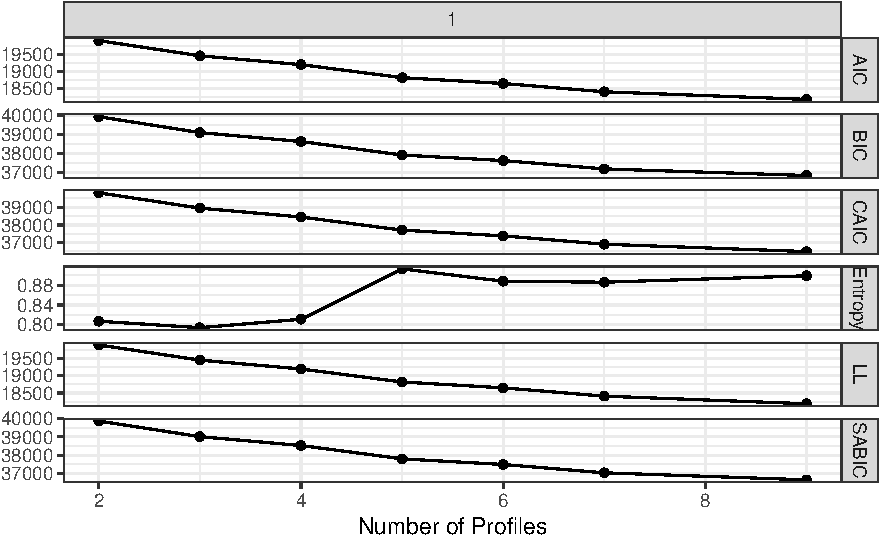
\includegraphics[width=0.6\linewidth]{rosenberg-dissertation_files/figure-latex/model1-1}

}

\caption{Fit statistics for model 1}\label{fig:model1}
\end{figure}

\begin{figure}

{\centering 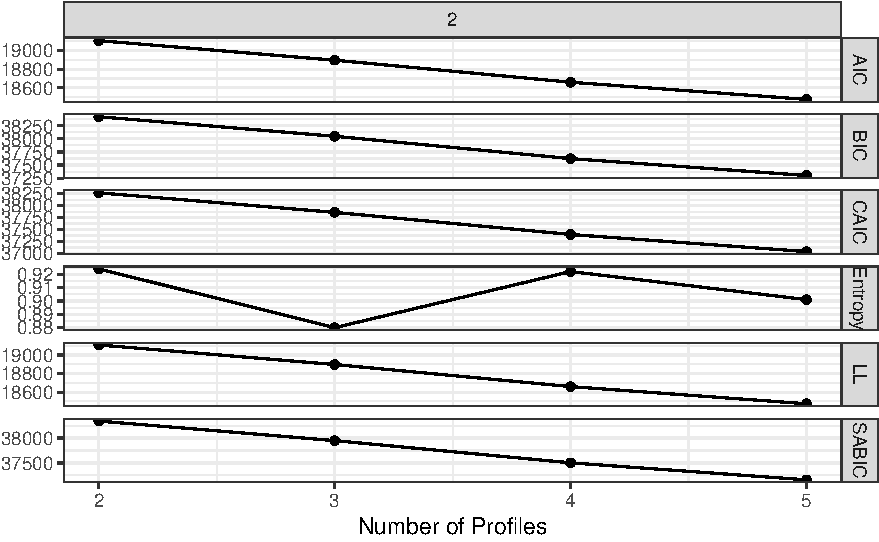
\includegraphics[width=0.5\linewidth]{rosenberg-dissertation_files/figure-latex/model2-1}

}

\caption{Fit statistics for model 2}\label{fig:model2}
\end{figure}

Looking across the statistics presented in Table 5.2 and Figures 5.1 and
5.2, some general ideas about which models are to be preferred emerge.
Solutions are interpreted first for each model individually and then
across models with the goal of choosing a smaller number of models to
investigate in more detail.

For solutions associated with model 1, the decrease (indicating a
preferred model) in information criteria becomes smaller as the number
of profiles increases from 5 to 6 and 6 to 7. A solution associated with
8 profiles did not replicate the log-likelihood and the VLMR and LMR
suggest that the solution associated with 9 profiles did not fit better
than that with 8 profiles, suggesting that models with 7 or fewer
profiles be preferred. Considering these models, the entropy statistic
increases by a large amount between the solution associated with 4 and 5
profiles (and then decreases slightly between 5 and 6 and 6 and 7
profile solutions), suggesting (but not providing conclusive evidence)
that models 5, 6, or 7 may be preferred. The bootstrapped LRT suggests
that, until the log-likelihood is not replicated, every more complex
model be selected. Taking these pieces of evidence into conclusion, for
model 1, solutions associated with 4 through 7 may be considered in more
depth, with an emphasis on solutions associated with profiles with 5 and
6 profiles on the basis of the slowing of the decrease in the
information criteria associated with the solutions with greater profiles
than these, and the increase in the entropy from 4 to 5 (and 6) profile
solutions.

For solutions associated with model 2, only those associated with 2-5
profile solutions were associated with log-likelihoods that were
replicated. For these four models, the log-likelihood decreased in a
mostly consistent way, such that changes in the decrease are not as
evident as those associated with model 1. The entropy statistic
decreases from 2 to 3 profile solutions, increases from 3 to 4 profile
solutions, and then decreases slightly from 4 to 5 profile solutions,
providing some information that models associated with 4 profiles be
preferred to the others. All of the LRTs suggest that the more complex
model be selected, not providing clear information about which solutions
are to be preferred. On the basis of these pieces of evidence, models
with 3, 4, and 5 solutions may be considered in more depth. However,
there is a lack of consistent evidence favoring more or less complex
models.

\subsection{Comparison of candidate
solutions}\label{comparison-of-candidate-solutions}

In this section, specific models are examined so that candidate
solutions can be compared. For all of the solutions, the data are
centered to have a mean equal to 0, but not scaled to have a standard
deviation equal to 1.

\subsection{Model 1 candidate
solutions}\label{model-1-candidate-solutions}

\subsubsection{Model: 1, Profiles: 3}\label{model-1-profiles-3}

This solution is characterized by:

\begin{itemize}
\tightlist
\item
  a \textbf{full} profile, profile 2 (though with more modestly high
  levels of challenge)
\item
  a \textbf{universally low} profile, profile 1 (again with more
  modestly - in this case low - levels of challenge)
\item
  an \textbf{all moderate} profile, profile 3, characterized by levels
  of all of the variables close to the mean, profile 3
\end{itemize}

The number of observations associated with each of the profiles is
somewhat balanced, with the all moderate profile demonstrating a higher
number of observations (\emph{n} = 1,288) than the full (\emph{n} = 897)
and universally low (\emph{n} = 773) profiles. The log-likelihood was
replicated many (more than 10) times. Because the profiles associated
with this solution all demonstrated the same overall pattern (i.e., all
five variables are high, low, or moderate), on the basis of
interpretability, this particular solution may not be useful in terms of
understanding how youth experience engagement and its conditions.

\begin{verbatim}
## Error in group_vars(x): object 'm1_3' not found
\end{verbatim}

\subsubsection{Model: 1, Profiles: 4}\label{model-1-profiles-4}

This solution is characterized by:

\begin{itemize}
\tightlist
\item
  a \textbf{full} profile, profile 2
\item
  a \textbf{universally low} profile, profile 1
\item
  an \textbf{all moderate} profile, profile 3.
\item
  a \textbf{competent but not engaged or challenged} profile, with high
  levels of challenge and low levels of engagement and competence
\end{itemize}

Most profiles are in the all moderate profile (\emph{n} = 1,288), with a
large number in the full (\emph{n} = 920) profile, and fewer in the
universally low and competent (\emph{n} n = 427) but not engaged or
challenged profiles (\emph{n} = 415). With somewhat more purchase in
terms of its interpretability than the solution for model 1 with three
profiles, like that solution, this one may not be as useful as more
complex models for understanding youth's experiences.

The log-likelihood was replicated many (more than 10) times.

\begin{verbatim}
## Error in group_vars(x): object 'm1_4' not found
\end{verbatim}

\subsubsection{Model: 1, Profiles: 5}\label{model-1-profiles-5}

This solution is characterized by:

\begin{itemize}
\tightlist
\item
  a \textbf{full} profile, profile 5
\item
  a \textbf{universally low} profile, profile 3
\item
  an \textbf{all moderate} profile, profile 3, though with moderate
  levels of affective engagement than in similar profiles associated
  with the four and five profile solutions, perhaps suggesting that a
  different profile than in those solutions
\item
  an **only behavioral* profile, profile 2, with moderate levels of
  behavioral engagement, very low affective engagement, and moderately
  (low) levels of cognitive engagement and challenge and competence
\item
  an \textbf{only affective} profile, profile 4, with moderate levels of
  affective engagement, low levels of behavioral engagement, and
  moderately (low) levels of cognitive engagement and challenge and
  competence
\end{itemize}

The number of observations associated with each of the profiles is
somewhat balanced, with a large number in the full profile (\emph{n} =
928), a moderate number of observations in the universally low (\emph{n}
= 667) and all moderate (\emph{n} = 643) profiles, and fewer
observations in the only behaviorally engaged (\emph{n} = 375) and only
affective engaged (\emph{n} = 345) profiles. This solution primarily
distinguishes between affective and behavioral engagement; unlike the
solution for model 1 with four profiles, there is not a competent but
not engaged or challenged profile. This may suggest that solutions with
a greater number of profiles represents both the distinction between
behavioral and affective engagement highlighted by profiles in this
solution as well as profiles that are characterized by higher or lower
levels of the conditions for engagement (i.e., competence). The
log-likelihood was replicated four times.

\begin{verbatim}
## Error in group_vars(x): object 'm1_5' not found
\end{verbatim}

\subsubsection{Model: 1, Profiles: 6}\label{model-1-profiles-6}

This solution is characterized by:

\begin{itemize}
\tightlist
\item
  a \textbf{full} profile, profile 6
\item
  a \textbf{universally low} profile, profile 2
\item
  an \textbf{all moderate} profile, profile 5--and, like, the model 1,
  six profile solution--with moderate levels of affective engagement
\item
  an \textbf{only behaviorally engaged} profile, profile 1, with
  moderate levels of behavioral engagement, very low affective
  engagement, and moderately (low) levels of cognitive engagement and
  challenge and competence
\item
  an \textbf{only affectively engaged} profile, profile 4, with moderate
  levels of affective engagement, low levels of behavioral engagement,
  and moderately (low) levels of cognitive engagement and challenge and
  competence
\item
  an \textbf{engaged and competent but not challenged} profile, profile
  3, characterized by high levels of each of the three dimensions of
  engagement and of competence, but with low levels of challenge
\end{itemize}

The number of observations associated with each of the profiles is
somewhat balanced, with the universally low profile with the largest
number of observations (\emph{n} = 667; the same number for this profile
as in the model 1, five profile solution), followed by the all moderate
profile (\emph{n} = 638). Each of the other four profiles were
associated with 300 to 400 observations. Unlike the model 1, four and
five profile solutions, which distinguished observations on
\emph{either} a condition of engagement (i.e., competence) or one of its
dimensions (i.e., cognitive, behavioral, and affective), this solution
was associated with profiles that distinguished observations on the
basis of both: There were profiles for only behaviorally and affectively
engaged and for engaged and competent but not challenged. While the
engaged and competent but not challenged was distinguished by low levels
of challenge--different from the profile associated with the model 1,
four profile solution characterized by high levels of competence--this
solution is compelling because it appears to group students on the basis
of multiple of the indicators, and demonstrate viability on the basis of
the fit statistics (i.e., Tables 5.1 and 5.2 and Figure 5.1). The
log-likelihood was replicated two times, with the next lowest
log-likelihood not being replicated, followed by a log-likelihood that
was replicated (at least) seven times. This solution (associated with
the log-likelihood that was replicated {[}at least{]} seven times) could
be investigated in further detail, to see whether--and if so, how--it
differs from the solution interpreted here. Pending further exploration,
this solution seems like a potential candidate for use in subsequent
analyses.

\begin{verbatim}
## Error in group_vars(x): object 'm1_6' not found
\end{verbatim}

\subsubsection{Model: 1, Profiles: 6
(alternate)}\label{model-1-profiles-6-alternate}

This solution is characterized by:

\begin{itemize}
\tightlist
\item
  a \textbf{full} profile, profile 6
\item
  a \textbf{universally low} profile, profile 1
\item
  an \textbf{engaged and competent but not challenged} profile, profile
  3
\item
  a \textbf{challenged} profile, profile 2
\item
  a \textbf{highly challenged} profile, profile 3
\item
  a \textbf{moderately low} profile, profile 5
\end{itemize}

The number of observations are not very balanced, with the moderately
low profile with a large number of observations (\emph{n} = 852) and the
challenged, engaged and competent but not challenged, and full profiles
with moderate numbers of observations (from 464 to 619 observations),
and low numbers of observations exhibited by universally low (\emph{n} =
280) and highly challenged (\emph{n} = 158) profiles. This--and,
critically, the lower log-likelihood of the other model 1, six profile
solution--suggests that this solution is not preferred. However, the
very different profiles that emerge for this solution suggest that there
might not be a somewhat under-identified solution associated with model
1 and six profiles.

\begin{verbatim}
## Error in group_vars(x): object 'm1_6_alt' not found
\end{verbatim}

\subsubsection{Model: 1, Profiles: 7}\label{model-1-profiles-7}

This solution is characterized by:

\begin{itemize}
\tightlist
\item
  a \textbf{full} profile, profile 7
\item
  a \textbf{universally low} profile, profile 1
\item
  a \textbf{competent but not engaged or challenged} profile, profile 2,
  characterized by high competence and moderate (low) or low levels of
  engagement and challenge
\item
  a \textbf{moderately low} profile, profile 3, characterized by
  moderately low levels of all of the variables
\item
  a \textbf{challenged} profile, profile 4, characterized by high
  challenge, moderate (high) levels of engagement, and moderate (low)
  levels of competence
\item
  a \textbf{highly challenged} profile, profile 5, characterized by
  patterns similar to those of the challenged profile, but with higher
  challenge and with low levels of both engagement and challenge
\item
  a \textbf{challenged but not engaged or competent} profile, profile 6,
  characterized by low levels of challenge, and high levels of
  engagement and competence
\end{itemize}

The number of observations associated with each of the profiles is not
very balanced, with few (\emph{n} = 181) observations associated with
the universally low profile and few (\emph{n} = 222) observations
associated with the highly challenged profile. The number of
observations associated with the other profiles ranged from 317 to 651.
Where the universally low profile exhibited the same number of
observations in the model 1, five and six profile solutions, for this
solution, there were far fewer observations. Also distinct from other
solutions, none of the other five profiles were found in the other model
1 solutions. Two pairs of the profiles--challenged and highly challenged
and universally low and moderately low--exhibited similar patterns among
the variables that were distinguished by different mean levels. The
log-likelihood was replicated twice, with the next lowest log-likelihood
being replicate four times, possibly warranting further investigation.
Taken together, this solution raises questions about whether it may be
too complex, possibly suggesting preference for model 1 five and six
profile solutions.

\begin{verbatim}
## Error in group_vars(x): object 'm1_7' not found
\end{verbatim}

\subsubsection{Model: 1, Profiles: 7
(alternate)}\label{model-1-profiles-7-alternate}

When investigating an alternate solution (associated with the second
lowest log-likelihood) for the model 1, seven profile solution, we can
see that even for the solutions associated with other log-likelihoods,
the profiles that can be identified are very similar. One minor
distinction concerns the \textbf{competent but not engaged or
challenged} profile, which in the alternate solution is associated with
neutral levels of affective engagement, compared to moderately low
levels of affective engagement in the solution with the lowest
log-likelihood. Because five of the seven profiles associated with both
of these model 1, seven profile solutions seem to be distinct from those
identified from simpler model 1 solutions, investigation of this
alternate solution provides additional evidence that these profiles are
not associated with an under-identified model and that simpler models
may be preferred over these seven profile solutions.

\begin{verbatim}
## Error in group_vars(x): object 'm1_7' not found
\end{verbatim}

\subsection{Model 2 candidate
solutions}\label{model-2-candidate-solutions}

\subsubsection{Model: 2, Profiles: 3}\label{model-2-profiles-3}

This solution is characterized by:

\begin{itemize}
\tightlist
\item
  a \textbf{universally low} profile, profile 1, associated with
  moderate (low) and low levels of all of the variables; this profile is
  similar to the universally low profile identified as part of other
  solutions, although with more moderate values for some of the
  variables (especially cognitive engagement)
\item
  a \textbf{competent but not challenged} profile, profile 2,
  characterized by high competence and low challenge
\item
  a \textbf{challenged} profile, profile 3, characterized by very high
  challenge and moderate (high) levels of the other variables, similar
  to the challenged profile found as part of the model 1, four profile
  solution, but with higher levels of competence, which are moderately
  high in this solution but moderately low for the other solution.
\end{itemize}

The number of observations associated with each solution is fairly
balanced, with the most in the challenged profile (\emph{n} = 1,241),
followed by the universally low (\emph{n} = 954 observations) and
competent but not challenged (\emph{n} = 763) profiles. This solution is
very different than the three profile solution that was interpreted for
model 1. Model 2 differs from model 1 in that covariances between the
variables are estimated (they are constrained to be the same are across
the profiles). The log-likelihood was replicated (at least) ten times.
Thus, this and other solutions associated with model 2 include
information about how the variables relate. Including this information
seems to be associated with profiles that differentiate the groups on
the basis of the levels of each of the variables in more distinct ways:
the model 1, three profile solution was characterized by high, moderate,
or low levels of all variables for each of the three profiles.

\begin{verbatim}
## Error in group_vars(x): object 'm2_3' not found
\end{verbatim}

\subsubsection{Model: 2, Profiles: 4}\label{model-2-profiles-4}

This solution is characterized by:

\begin{itemize}
\tightlist
\item
  a \textbf{universally low} profile, profile 1
\item
  a \textbf{challenged} profile, profile 2
\item
  a \textbf{highly challenged} profile, profile 4
\item
  an \textbf{engaged and competent but not challenged} profile, profile
  3
\end{itemize}

The number of observations in each of the profiles is not very balanced,
with more than 1,000 observations in both the universally low (\emph{n}
= 1,029) and challenged (\emph{n} = 1,106) profiles, a moderate number
if the engaged and competent but not challenged profile (\emph{n} =
688), and very few in the highly challenged (\emph{n} = 135) profile.
The log-likelihood was replicated three times. While each of these
profiles has been identified in another solution, the small number of
observations in the highly challenged profile suggests that this
solution be interpreted with some skepticism because of the potentially
limited utility (and statistical power associated with the use) of the
profiles in subsequent analyses.

\begin{verbatim}
## Error in group_vars(x): object 'm2_4' not found
\end{verbatim}

\subsubsection{Model: 2, Profiles: 5}\label{model-2-profiles-5}

This solution is characterized by:

\begin{itemize}
\tightlist
\item
  a \textbf{universally low} profile, profile 1
\item
  a \textbf{full} profile, profile 4, although with very high levels of
  challenged (in addition to high levels of all of the other variables),
  making this profile similar to that (challenged) profile
\item
  a \textbf{highly challenged} profile, profile 5
\item
  an \textbf{all moderate} profile, profile 3, although with moderately
  lower levels of competence than is found in profiles associated with
  other solutions
\item
  a \textbf{competent but not challenged} profile, profile 2, similar to
  the competent but not challenged or engaged profile, but with neutral,
  rather than low, levels of the engagement variables
\end{itemize}

The number of observations associated with each of the profiles is not
very balanced, with a very large number of observations in the all
moderate profile (\emph{n} = 1,113) and a large number in the competent
but not challenged profile (\emph{n} = 871), a moderate number in the
full profile (\emph{n} = 573), and very few in the universally low
(\emph{n} = 271) and challenged but not competent (\emph{n} = 130)
profiles. The log-likelihood was replicated four times. Like for the
model 2, four profile solution, the small number of observations
associated with two of the profiles suggests that this solution should
be interpreted with some caution.

\begin{verbatim}
## Error in group_vars(x): object 'm2_5' not found
\end{verbatim}

\subsubsection{Looking across model 1 and model 2
solutions}\label{looking-across-model-1-and-model-2-solutions}

When looking across solutions, some overall patterns in terms of what
profiles emerge and some directions for which models are to be selected
for use in subsequent analysis can be identified. First, overall
patterns are discussed. In table 5.3, which profiles emerge from which
solution is presented.

There is a wide range of profiles. Some appear very commonly,
particularly those (full and universally low) characterized by high or
low levels across all of the variables.

\begin{landscape}\begin{table}

\caption{\label{tab:compare-profiles-by-solution}Profile assignments by LPA solution}
\centering
\resizebox{\linewidth}{!}{\begin{tabular}[t]{rlllllllllllll}
\toprule
Model & Number of Profiles & Full & All Moderate & Comptent but not Engaged or Challenged & Only Behavioral & Only Affective & Moderately Low & Engaged and Competent but not Challenged & Challenged but not Engaged or Comptent & Challenged & Highly Challenged & Universally Low & Comptent but not Challenged\\
\midrule
1 & 3 & x & x & NA & NA & NA & NA & NA & NA & NA & NA & x & NA\\
1 & 4 & x & x & NA & NA & NA & NA & NA & NA & NA & NA & x & x\\
1 & 5 & x & x & NA & x & x & NA & NA & NA & NA & NA & x & NA\\
1 & 6 & x & x & NA & x & x & NA & x & NA & NA & NA & x & NA\\
1 & 6 (alt) & x & NA & NA & NA & NA & x & x & NA & x & x & x & NA\\
1 & 7 & x & NA & NA & NA & NA & x & NA & x & x & x & x & x\\
1 & 7 (alt) & x & NA & NA & NA & NA & x & NA & x & x & x & x & x\\
2 & 3 & NA & NA & NA & NA & NA & NA & NA & NA & x & NA & x & x\\
2 & 4 & NA & NA & NA & NA & NA & NA & x & NA & x & x & x & NA\\
2 & 5 & x & x & NA & NA & NA & NA & NA & NA & NA & x & x & x\\
\bottomrule
\end{tabular}}
\end{table}
\end{landscape}

The model 1, six and seven profile solutions are compelling because both
show profiles that are distinguished by dimensions of engagement and its
conditions (challenge and competence). For each solution, alternate
solutions associated with higher log-likelihoods were explored. One
advantage of the six profile solution is that most of its profiles can
also be identified in solutions with fewer profiles. For the six profile
solutions, this alternate solution was very different, whereas for the
seven profile solutions, this alternate solution was highly similar. The
model solutions exhibit a less clear pattern in terms of which profiles
appear when. All else being equal, on the basis of parsimony, the model
1, six profile solution may be preferred. As a type of sensitivity
analysis, the model 1, seven profile solution is also explored, but
results for it are included in an appendix.

\section{Research Question \#2}\label{research-question-2}

Research question \#2 is focused on the relations between each of the
profiles and the aspects of work with data.

\section{Research Question \#3}\label{research-question-3}

Research question \#3 is focused on

\section{Research Question \#4}\label{research-question-4}

Research question \#4 is focused on

\chapter{Discussion}\label{discussion}

\chapter{References}\label{references}

Akiva, T. (2005). Turning training into results: The new youth program
quality assessment. High/Scope Resource, 24(2), 21-24.\\
Bergman, L. R., \& Magnusson, D. (1997). A person-oriented approach in
research on developmental psychopathology. Development and
psychopathology, 9(2), 291-319.\\
Bergman, L. R., Magnusson, D., \& El Khouri, B. M. (2003). Studying
individual development in an interindividual context: A person-oriented
approach. Psychology Press.\\
Berland, L. K., Schwarz, C. V., Krist, C., Kenyon, L., Lo, A. S., \&
Reiser, B. J. (2016). Epistemologies in practice: Making scientific
practices meaningful for students. Journal of Research in Science
Teaching, 53(7), 1082-1112.\\
Bielik, T., \& Yarden, A. (2016). Promoting the asking of research
questions in a high-school biotechnology inquiry-oriented program.
International Journal of STEM Education, 3(1), 15.\\
Breckenridge, J. N. (2000). Validating cluster analysis: Consistent
replication and symmetry. Multivariate Behavioral Research, 35(2),
261-285.\\
Bystydzienski, J. M., Eisenhart, M., \& Bruning, M. (2015). High school
is not too late: Developing girls' interest and engagement in
engineering careers. Career Development Quarterly, 63(1), 88--95.
\url{http://doi.org/10.1002/j.2161-0045.2015.00097.x} Cohen, J. (1992).
A power primer. Psychological Bulletin, 112(1), 155.\\
National Governors Association Center for Best Practices, Council of
Chief State School Officers. (2010). Common Core State Standards for
Mathematics. Washington, DC: National Governors Association Center for
Best Practices and the Council of Chief State School Officers.\\
Corpus, J. H., \& Wormington, S. V. (2014). Profiles of intrinsic and
extrinsic motivations in elementary school: A longitudinal analysis. The
Journal of Experimental Education, 82(4), 480-501.\\
Csikszentmihalyi, M. (1990). Flow: The psychology of optimal
performance. Cambridge, England: Cambridge University Press.\\
Csikszentmihalyi, M. (1997). Finding flow: The psychology of engagement
with everyday life. New York, NY: Basic Books.\\
Creswell, J. W., Plano Clark, V. L., Gutmann, M. L., \& Hanson, W. E.
(2003). Advanced mixed methods research designs. In A. Tashakkori \& C.
Teddlie (Eds.), Handbook of mixed methods in social and behavioral
research (pp.~209--240). Thousand Oaks, CA: Sage.\\
English, L. D. (2012). Data modelling with first-grade students.
Educational Studies in Mathematics, 81(1), 15-30.\\
Finzer, W. (2013). The data science education dilemma. Technology
Innovations in Statistics Education, 7(2), p.~1-9.\\
Franklin, C., Kader, G., Mewborn, D., Moreno, J., Peck, R., Perry, M.,
\& Scheaffer, R. (2007). Guidelines for assessment and instruction in
statistics education (GAISE) report. Alexandria, VA: American
Statistical Association.\\
Fredricks, J. A., \& McColskey, W. (2012). The measurement of student
engagement: A comparative analysis of various methods and student
self-report instruments. In S. L. Christenson, A. L. Reschly, \& C.
Wylie (Eds.), The handbook of research on student engagement
(pp.~763--782). New York: Springer Science.
\url{https://doi.org/10.1007/978-1-4614-2018-7_37}\\
Fredricks, J. A., Blumenfeld, P. C., \& Paris, A. H. (2004). School
engagement: Potential of the concept, state of the evidence. Review of
Educational Research, 74(1), 59-109.\\
Fredricks, J. A., Filsecker, M., \& Lawson, M. A. (2016). Student
engagement, context, and adjustment: Addressing definitional,
measurement, and methodological issues. Learning \& Instruction, 43,
1-4.\\
Gelman, S. A., \& Markman, E. M. (1987). Young children's inductions
from natural kinds: The role of categories and appearances. Child
Development, 58(6), 1532-1541.\\
Gopnik, A., \& Sobel, D. M. (2000). Detecting blickets: How young
children use information about novel causal powers in categorization and
induction. Child Development, 71(5), 1205-1222.\\
Gopnik, A., Sobel, D. M., Schulz, L. E., \& Glymour, C. (2001). Causal
learning mechanisms in very young children: two-, three-, and
four-year-olds infer causal relations from patterns of variation and
covariation. Developmental Psychology, 37(5), 620.\\
Greene, B. A. (2015). Measuring cognitive engagement with self-report
scales: Reflections from over 20 years of research. Educational
Psychologist, 50(1), 14-30.\\
Greene, K. M., Lee, B., Constance, N., \& Hynes, K. (2013). Examining
youth and program predictors of engagement in out-of-school time
programs. Journal of Youth and Adolescence, 42(10), 1557-1572.\\
Hancock, C., Kaput, J. J., \& Goldsmith, L. T. (1992). Authentic inquiry
with data: Critical barriers to classroom implementation. Educational
Psychologist, 27(3), 337-364.\\
Harring, J. R., \& Hodis, F. A. (2016). Mixture modeling: Applications
in educational psychology. Educational Psychologist, 51(3-4), 354-367.\\
Hasson, E., \& Yarden, A. (2012). Separating the research question from
the laboratory techniques: Advancing high‐school biology teachers'
ability to ask research questions. Journal of Research in Science
Teaching, 49(10), 1296-1320.\\
Hayenga, A. O., \& Corpus, J. H. (2010). Profiles of intrinsic and
extrinsic motivations: A person-centered approach to motivation and
achievement in middle school. Motivation and Emotion, 34(4), 371-383.\\
Hektner, J. M., Schmidt, J. A., \& Csikszentmihalyi, M. (2007).
Experience sampling method: Measuring the quality of everyday life.
Sage.\\
Jahnukainen, M. (2010). Extreme cases. Encyclopedia of Case Study
Research. Thousand Oaks, CA: Sage.\\
Konold, C., \& Pollatsek, A. (2002). Data analysis as the search for
signals in noisy processes. Journal for Research in Mathematics
Education, 33(4), 259-289.\\
Lauer, P. A., Akiba, M., Wilkerson, S. B., Apthorp, H. S., Snow, D., \&
Martin-Glenn, M. L. (2006). Out-of-school-time programs: A meta-analysis
of effects for at-risk students. Review of educational research, 76(2),
275-313.\\
Lee, H. S., Angotti, R. L., \& Tarr, J. E. (2010). Making comparisons
between observed data and expected outcomes: students' informal
hypothesis testing with probability simulation tools. Statistics
Education Research Journal, 9(1), 68-96.\\
Lee, H., \& Hollebrands, K. (2008). Preparing to teach mathematics with
technology: An integrated approach to developing technological
pedagogical content knowledge. Contemporary Issues in Technology and
Teacher Education, 8(4), 326-341.\\
Lehrer, R., \& Romberg, T. (1996). Exploring children's data modeling.
Cognition and Instruction, 14(1), 69-108.\\
Lehrer, R., \& Schauble, L. (2004). Modeling natural variation through
distribution. American Educational Research Journal, 41(3), 635-679.\\
Lehrer, R. \& Schauble, L. (2015). Developing scientific thinking. In L.
S. Liben \& U. Müller (Eds.), Cognitive processes. Handbook of child
psychology and developmental science (Vol. 2, 7th ed., pp.~671-174).
Hoboken, NJ: Wiley.\\
Lehrer, R., Kim, M. J., \& Jones, R. S. (2011). Developing conceptions
of statistics by designing measures of distribution. ZDM, 43(5),
723-736.\\
Lehrer, R., Kim, M. J., \& Schauble, L. (2007). Supporting the
development of conceptions of statistics by engaging students in
measuring and modeling variability. International Journal of Computers
for Mathematical Learning, 12(3), 195-216.\\
Lesh, R., Middleton, J. A., Caylor, E., \& Gupta, S. (2008). A science
need: Designing tasks to engage students in modeling complex data.
Educational Studies in Mathematics, 68(2), 113-130.\\
Linnansaari, J., Viljaranta, J., Lavonen, J., Schneider, B., \&
Salmela-Aro, K. (2015). Finnish Students Engagement in Science Lessons.
NorDiNa: Nordic Studies in Science Education, 11(2), 192-206. Retrieved
from
\url{https://www.journals.uio.no/index.php/nordina/article/view/2047}\\
Lovett, M. C., \& Shah, P. (2007). Preface. In M. C. Lovett \& P. Shah
(Eds.), Thinking with data (pp.~x-xx {[}requested book through ILL to
confirm page \#s{]}). New York, NY: Lawrence Erlbaum.\\
Magnusson, D., \& Cairns, R. B. (1996). Developmental science: Toward a
unified framework. Cambridge, England: Cambridge University Press.\\
McNeill, K. L., \& Berland, L. (2017). What is (or should be) scientific
evidence use in k‐12 classrooms? Journal of Research in Science
Teaching, 54(5), 672-689.\\
Muthén, B. (2004). Latent variable analysis. The Sage handbook of
quantitative methodology for the social sciences. Thousand Oaks, CA:
Sage Publications, 345-68.\\
Muthén, L. K., \& Muthén, B. O. (1998-2017). Mplus User's Guide. Los
Angeles, CA: Muthén \& Muthén. NGSS Lead States. (2013). Next generation
science standards: For states, by states. Washington, DC: National
Academies Press.\\
Nolen, S. B., Horn, I. S., \& Ward, C. J. (2015). Situating motivation.
Educational Psychologist, 50(3), 234-247. Patall, E. A., Vasquez, A. C.,
Steingut, R. R., Trimble, S. S., \& Pituch, K. A. (2016). Daily
interest, engagement, and autonomy support in the high school science
classroom. Contemporary Educational Psychology, 46, 180-194.\\
Patall, E. A., Steingut, R. R., Vasquez, A. C., Trimble, S. S., Pituch,
K. A., \& Freeman, J. L. (2017). Daily Autonomy Supporting or Thwarting
and Students' Motivation and Engagement in the High School Science
Classroom. Journal of Educational Psychology. Advance online
publication. \url{http://dx.doi.org/10.1037/edu0000214}\\
Pekrun, R., \& Linnenbrink-Garcia, L. (2012). Academic emotions and
student engagement. In S. L. Christenson, A. L. Reschly, \& C. Wylie
(Eds.), Handbook of research on student engagement (pp.~259-292). New
York, NY: Springer. Petrosino, A., Lehrer, R., \& Schauble, L. (2003).
Structuring error and experimental variation as distribution in the
fourth grade. Mathematical Thinking and Learning, 5 (2\&3), 131-156.\\
Piaget, J., \& Inhelder, B. (1969). The psychology of the child. New
York, NY: Basic Books.\\
Pöysä, S., Vasalampi, K., Muotka, J., Lerkkanen, M. K., Poikkeus, A. M.,
\& Nurmi, J. E. (2017). Variation in situation-specific engagement among
lower secondary school students. Learning and Instruction.
\url{http://dx.doi.org/10.1016/j.learninstruc.2017.07.007}\\
Rosenberg, J. M. (2018). Comparing mplus and mclust output. Retrieved
from
\url{https://jrosen48.github.io/r-markdown/comparing-mplus-mclust.html}
Salmela-Aro, K., Moeller, J., Schneider, B., Spicer, J., \& Lavonen, J.
(2016). Integrating the light and dark sides of student engagement using
person-oriented and situation-specific approaches. Learning and
Instruction, 43, 61-70.\\
Salmela-Aro, K., Muotka, J., Alho, K., Hakkarainen, K., \& Lonka, K.
(2016). School burnout and engagement profiles among digital natives in
Finland: A person-oriented approach. European Journal of Developmental
Psychology, 13(6), 704-718.\\
Schneider, B., Krajcik, J., Lavonen, J., Salmela‐Aro, K., Broda, M.,
Spicer, J., \ldots{} \& Viljaranta, J. (2016). Investigating optimal
learning moments in US and Finnish science classes. Journal of Research
in Science Teaching, 53(3), 400-421.\\
Schmidt, J. A., Rosenberg, J. M., Beymer, P. (advance online
publication). A person-in-context approach to student engagement in
science: Examining learning activities and choice. Journal of Research
in Science Teaching. \url{https://dx.doi.org/10.1002/tea.21409}\\
Schwarz, N., Kahneman, D., \& Xu, J. (2009). Global and episodic reports
of hedonic experience. In R. Belli, D. Alwen, \& F. Stafford (Eds.),
Using calendar and diary methods in life events research (pp.~157-174).
Newbury Park, CA: Sage.\\
Sfard, A. (1998). On two metaphors for learning and the dangers of
choosing just one. Educational Researcher, 27(2), 4-13.\\
Shernoff, D. J., Csikszentmihalyi, M., Schneider, B., \& Shernoff, E. S.
(2003). Student engagement in high school classrooms from the
perspective of flow theory. School Psychology Quarterly, 18(2),
158-176.\\
Shernoff, D. J., Kelly, S., Tonks, S. M., Anderson, B., Cavanagh, R. F.,
Sinha, S., \& Abdi, B. (2016). Student engagement as a function of
environmental complexity in high school classrooms. Learning and
Instruction, 43, 52-60.\\
Shumow, L., \& Schmidt, J. A. (2013). STEM interest and engagement (STEM
I.E.). National Science Foundation proposal for award number 1421198.\\
Sinatra, G. M., Heddy, B. C., \& Lombardi, D. (2015). The challenges of
defining and measuring student engagement in science. Educational
Psychologist, 50(1), 1-13. \url{doi:10.1080/00461520.2014.1002924}\\
Singh, K., Granville, M., \& Dika, S. (2002). Mathematics and science
achievement: Effects of motivation, interest, and academic engagement.
The Journal of Educational Research, 95(6), 323-332.\\
Shernoff, D. J., \& Schmidt, J. A. (2008). Further Evidence of an
Engagement--Achievement Paradox Among U.S. High School Students. Journal
of Youth and Adolescence, 37(5), 564--580.
\url{http://doi.org/10.1007/s10964-007-9241-z}\\
Shumow, L., Schmidt, J. A., \& Zaleski, D. J. (2013). Multiple
perspectives on student learning, engagement, and motivation in high
school biology labs. The High School Journal, 96(3), 232-252.\\
Skinner, E. A., \& Pitzer, J. (2012). Developmental dynamics of
engagement, coping, and everyday resilience. In S. Christenson, A.
Reschly, \& C. Wylie (Eds.), Handbook of Research on Student Engagement
(pp.~21-45). New York: Springer Science.\\
Skinner, E. A., Kindermann, T. A., \& Furrer, C. J. (2009). A
motivational perspective on engagement and disaffection:
Conceptualization and assessment of children's behavioral and emotional
participation in academic activities in the classroom. Educational and
Psychological Measurement, 69(3), 493-525.\\
Skinner, E., Furrer, C., Marchand, G., \& Kindermann, T. (2008).
Engagement and disaffection in the classroom: Part of a larger
motivational dynamic? Journal of Educational Psychology, 100(4), 765.\\
Steinley, D., \& Brusco, M. J. (2011). Evaluating mixture modeling for
clustering: recommendations and cautions. Psychological Methods, 16(1),
63.\\
Stohl, H., \& Tarr, J. E. (2002). Developing notions of inference using
probability simulation tools. The Journal of Mathematical Behavior,
21(3), 319-337.\\
Stroupe, D. (2014). Examining classroom science practice communities:
How teachers and students negotiate epistemic agency and learn
science‐as‐practice. Science Education, 98(3), 487-516.\\
Strati, A. D., Schmidt, J. A., \& Maier, K. S. (2017). Perceived
challenge, teacher support, and teacher obstruction as predictors of
student engagement. Journal of Educational Psychology, 109(1),
131-147.\\
Trevors, G. J., Kendeou, P., Bråten, I., \& Braasch, J. L. (2017).
Adolescents' epistemic profiles in the service of knowledge revision.
Contemporary Educational Psychology, 49, 107-120.\\
Turner, J. C., \& Meyer, D. K. (2000). Studying and understanding the
instructional contexts of classrooms: Using our past to forge our
future. Educational Psychologist, 35(2), 69-85.\\
van Rooij, E. C., Jansen, E. P., \& van de Grift, W. J. (2017).
Secondary school students' engagement profiles and their relationship
with academic adjustment and achievement in university. Learning and
Individual Differences, 54, 9-19.\\
Vandell, D. L., Hall, V., O'Cadiz, P., \& Karsh, A. (2012). Piloting
outcome measures for summer learning initiative programs. Final report
to the David and Lucile Packard Foundation, Children, Families, and
Communities Program. Retrieved from
\url{http://faculty.sites.uci.edu/childcare/files/2013/07/SL-Outcomes-2011-Pilot_Edited_8.19.pdf}\\
Wang, M. T., \& Eccles, J. S. (2012). Social support matters:
Longitudinal effects of social support on three dimensions of school
engagement from middle to high school. Child Development, 83(3),
877-895.\\
Wang, M. T., \& Holcombe, R. (2010). Adolescents' perceptions of school
environment, engagement, and academic achievement in middle school.
American Educational Research Journal, 47(3), 633-662.\\
Westfall, J., Kenny, D. A., \& Judd, C. M. (2014). Statistical power and
optimal design in experiments in which samples of participants respond
to samples of stimuli. Journal of Experimental Psychology: General,
143(5), 2020-2045.\\
Westfall, J. (2016). PANGEA: Power Analysis for General Anova designs.
Retrieved from \url{https://jakewestfall.shinyapps.io/pangea/}\\
Wickham, H. (2018). CRAN downloads. Retrieved from
\url{https://hadley.shinyapps.io/cran-downloads/} Wild, C. J., \&
Pfannkuch, M. (1999). Statistical thinking in empirical enquiry.
International Statistical Review, 67(3), 223-248.\\
Wilkerson, M. H., Andrews, C., Shaban, Y., Laina, V., \& Gravel, B. E.
(2016). What's the technology for? Teacher attention and pedagogical
goals in a modeling-focused professional development workshop. Journal
of Science Teacher Education, 27(1), 11-33.\\
Wilkerson, M. H. \& Fenwick, M. (2017). The practice of using
mathematics and computational thinking. In C. V. Schwarz, C. Passmore,
\& B. J. Reiser (Eds.), Helping Students Make Sense of the World Using
Next Generation Science and Engineering Practices. Arlington, VA:
National Science Teachers' Association Press. pp.~181-204.\\
Witherington, D. C. (2015). Dynamic systems in developmental science. In
W. F. Overton \& P. C. M. Molenaar (Vol. Eds.) \& R. M. Lerner (Ed.),
Handbook of child psychology and developmental science. Vol. 1: Theory
\& method (7th ed., pp.~63-112). Hoboken, NJ: Wiley.\\
Wormington, S. V., \& Linnenbrink-Garcia, L. (advance online
publication). A new look at multiple goal pursuit: The promise of a
person-centered approach. Educational Psychology Review.
\url{doi:10.1007/s10648-016-9358-2}

\bibliography{book.bib,packages.bib}


\end{document}
